\documentclass[a4paper,openright,12pt]{book}
\usepackage[utf8]{inputenc}
\usepackage{graphicx,color}
\usepackage[dvipsnames]{xcolor}
\usepackage{amsfonts}
\usepackage{amsmath}
\usepackage{amssymb}
\usepackage{verbatim}
\usepackage{cite} 
\usepackage{fancyhdr}
\usepackage{epigraph}
\graphicspath{{./figures/}}
%To use a kind of times new roman font style
\usepackage{mathptmx}
\usepackage{newtxtext,newtxmath}
%To modify the space before title of each chapter
%\usepackage{titlesec}
%\titleformat{\chapter}[display]   
%{\normalfont\huge\bfseries}{\chaptertitlename\ \thechapter}{20pt}{\Huge}   
%\titlespacing*{\chapter}{0pt}{-10pt}{40pt}
%Modificar encabezado y pie de página.
\pagestyle{fancy}
\fancyhead{}
\fancyhead[LE,RO]{\thepage}
\fancyhead[RE]{Nanoscale hydrodynamics near solids}
\fancyhead[LO]{{\color{Gray}CHAPTER \thechapter.} \leftmark }
\fancyfoot{}
%\fancyfoot[LE,RO]{\thepage}
%\fancyfoot[LO,CE]{Chapter \thechapter}
%\fancyfoot[CO,RE]{Author Name}
%New commands
\renewcommand{\thefootnote}{\roman{footnote}}
\newcommand{\esc}{\!\cdot\!}
\newcommand{\Note}[1]{{\bf \color{red}#1}}    % comments and notes
\newcommand{\Cambio}[1]{{\color{blue}#1}}     % cambio con respecto a los artículos
\newcommand{\Pendiente}[1]{{\color{green}#1}} % pendiente
\newcommand{\Tirar}[1]{{\color{Magenta}#1}}   % tirar
\newcommand{\llangle}{\left\langle}
\newcommand{\rrangle}{\right\rangle}

\begin{document}

\begin{titlepage}
\begin{center}
\begin{Huge}
\textsc{Nanoscale hydrodynamics \\ near solids}
\end{Huge}
\end{center}
\end{titlepage}


\newpage
$\ $
\thispagestyle{empty} % para que no se numere esta pagina


\chapter*{}
\pagenumbering{Roman} % para comenzar la numeracion de paginas en numeros romanos
\begin{flushright}
blablabla
\end{flushright}

\chapter*{Acknowledgments} % si no queremos que añada la palabra "Capitulo"
%\addcontentsline{toc}{chapter}{Agradecimientos} % si queremos que aparezca en el índice
\markboth{Acknowledgments}{Acknowledgments} % encabezado 
blablabla


\chapter*{Abstract} % si no queremos que añada la palabra "Capitulo"
%\addcontentsline{toc}{section}{Abstract} % si queremos que aparezca en el índice
\markboth{Abstract}{Abstract} % encabezado
blablabla


\chapter*{Resumen} % si no queremos que añada la palabra "Capitulo"
%\addcontentsline{toc}{section}{Resumen} % si queremos que aparezca en el índice
\markboth{RESUMEN}{RESUMEN} % encabezado
blablabla

\tableofcontents % indice de contenidos

\pagenumbering{arabic}
\setcounter{chapter}{-1}
\chapter{Introduction}\label{cap.Intro}
\markboth{Introduction}{Introduction}

%CHAPTER 1
\chapter{Nonequilibrium Statistical Mechanics}\label{cap.NESM}
\markboth{Nonequilibrium Statistical Mechanics}{}
\epigraph{\textit{There is no future. There is no past. Do you see? Time is simultaneous, an intricately structured jewel that humans insist on viewing one edge at a time, when the whole design is visible in every facet.}}{Watchmen \\ ALAN MOORE}

\section{Introduction}
It was in the nineteen century when the Statistical Mechanics (SM) was born mainly because of the work of Ludwing Boltzmann (1844-1906) and Josiah Willard Gibbs (1839-1903). The goal was to reconcile the Thermodynamics with the microscopic laws. 

Thermodynamics was well-established because it draws its concepts from experiments while the attemps to understand it from the Newton's laws collided with problems such as the imposibility of taking into account the interactions between all the particles of a thermodynamic system, the highly nontrivial of theses interactions, the huge number of degrees of freedom or the Loschmidt's paradox\footnote{The second law of thermodynamics estabishes that the entropy of an isolated system increases with time. This can be understood as a time direction imposed by the increasing of the entropy. Furthermore, Newton's laws are reversible. According to Josef Loschmidt (1821-1895) this apparently conflict could be the responsible of the imposibility to derive the laws of the thermodynamics from the microscopic laws.}. 
To avoid these problems physicist realized that the macro properties of a thermodynamic system does not strongly depend on the exact dynamics of every particle, but more on the averages that eventually polish the details of the behaviour of the particles. 
Thus, the link between the microscopic and macroscopic theory of matter can be stated appling statistical techniques to the microscopical mechanics laws. 
The connection is posible to the notion of ensemble, which is a collection of imaginary systems with a set of common macroscopic properties.  

In this way we may define Statistical Mechanics as a theoretical framework which allows to study the macro-properties of a many-body system from the dynamics of its microcopic constituents.
Therefore, we may roughly say that Statistical Mechanics acts as a bridge between two levels of description: microscopic level governed by the Newton's laws of motion and the macroscopic level where which is measure with experiments.
A beautiful but rough example about how Statistical Mechanics works can be found in the latter book of Dean Rickles, {\it Philosophy of Physics} \cite{Rickles2016}.
He imagines a large musical ensemble playing in concert.
The "global" sound produced by the musicians is analogue to the thermodynamic variables obtained from the colisions between the particles in the system. 
The music can me analized from two levels: the global level, where the harmony and the musical form take an important role, and the individual level, in which we focus in what the musicians are playing to produce the global sound. "In this zooming in and out", in words of Rickles, "from the whole system to its parts, that characterizes the relationship between statistical mechanics and thermodynamics: you won't see harmonies in a single bassoon; likewise, you won't see pressure or temperature in an individual molecule."

In this chapter, we review fundamental concepts of SM such as phase space, phase point and phase trajectory.
We introduce from Classical Mechanics (CM) the Hamilton's equations to describe the time evolution of a phase point in the phase space. 
Because of the non-linearity of these equations we write them in the language of the linear operators, where the Liouville operator $i{\rm L}$ plays an important role in the dynamics of the microstates. 
This techniques allows us to obtain the Hamilton's equations as first order differential equations. 
With these equations the trajectory of a phase point is deterministic, but we can not avoid the fact that we have no access to the position and momenta of all particles of the system. 
We introduce the concept of probability density in order to take into account our lack of knowledge of the initial condition. 
Therefore, the evolution of a phase point in the phase space converts into a stochastic process where the evolution of the probability density  is governed by the Liouville equation.
We review the Lioville theorem that tell us that the evolution of a bunch of phase point inside a volume must be conserved (i.e. the volumen must be the same but not the shape). 

In this chapter, we will review the Theory of Coarse-Graining (ToCG) which allows one to describe the dynamics with variables that capture the essential information of the system. 
These variables are called Coarse-Grained variables (CG variables) and evolve much more slowy than the neglected variables. 

Finally, we will introduce the time-dependent projection operator technique to derive the evolution equation of the CG variables. This technique is an aproximation of the time dependent ensemble, solution of the Liouville equation, with a relevant ensemble plus a correction responsible of the irreversible behaviour. This relevant ensemble is obtained maximizing the entropy functional of Gibbs-Jaynes. 


\section{Hamilton's equations and the evolution of the microstates}
Consider a system consisting of $N$ particles of mass $m$ in a volume $V$. In Classical Mechanics the positions of the particles ${\bf q}^N\equiv ({\bf q}_1,\dots,{\bf q}_N)^T$ and their 3N momenta ${\bf p}^N\equiv ({\bf p}_1,\dots,{\bf p}_N)^T$ specify the state of the system at any time. 
The collection of the positions and momenta of the particles defines the microscopic state of the system $z=(q,p)^T$. which is a phase point in the phase space $\Gamma$ of 6N dimensions. The notation emphasized that $z$ is a column vector, where $T$ is the transpose. Therefore, the time evolution of a phase point $z_t$ is called the phase trajectory and it is determined by the Hamilton's equations of motion

\begin{equation}
    \dot{{\bf q}}_i = \frac{\partial \hat{H}}{\partial {\bf p}_i}, \dot{{\bf p}}_i = -\frac{\partial \hat{H}}{\partial {\bf q}_i}
  \label{HamiltonEqs}
\end{equation}

Typically the Hamiltonian has the form
\begin{align}
    \hat{H}(z) = \sum_{i=1}^{N}\frac{{\bf p}_i^2}{2m}+\hat{U}({\bf q}_1,\dots,{\bf q}_N)+\sum_{i=1}^{N}\Phi({\bf q}_i),
\end{align}

where the first sum is the kinetic energy of the system, the potential of interaction
between particles is $\hat{U}({\bf q}_1,\dots,{\bf q}_N)$ and $\Phi({\bf r})$ is a time-independent external potential. 


Note that the the phase trajectories can not pass through the same point of the phase space because the evolution of the phase point is subject to 6N initial conditions. 
Thus, if two trajectories in phase space cross is because they started at the same phase point.  


Hamilton's equations can be written in compact form as
\begin{align}
  \dot{z}_t = J\cdot\frac{\partial\hat{H}}{\partial{z}}(z_t)\equiv \hat{v}(z_t),
  \label{compactHamiltonEqs}
\end{align}

where we have defined the Hamiltonian vector field $\hat{v}(z_t)$ and $J$ is the symplectic matrix\footnote{J is an orthogonal matriz, $J^TJ=1\to J^T = J^{-1}$, and its square is the minus the identity matrix $J^2=-1$} with the form
$$
\begin{pmatrix} 
  0 & 1_{3N} \\
  -1_{3N} & 0 
\end{pmatrix},
$$
where $1_{3N}$ is the identity matrix of dimension $3N \times 3N$.

Hamilton's equation (\ref{compactHamiltonEqs}) indicates that the trajectory of $z_t$ in phase space is an integral curve of the velocity field. Therefore, if we follow the indications given by the velocity field we can figure out which microstate will be the next one. 


\subsection{Linear Hamilton's equations}
In the last section we have presented Hamilton's equations as a set of \Note{non-linear ordinary differential equations}. However, in the language of linear operators we may obtain linear equations that are amenable of theoretical treatment. 
By analogy with Quantum Mechanics we consider all functions $\hat{B}(z)$ in phase space as a Hilbert vector space. Each function $\hat{B}(z)$ is a vector in the infinite-dimensional Hilbert space vector. As well as the state vector in Quantum Mechanics, $|\Psi\rangle$, each function (vector) $\hat{B}$ has the dimension of all the possible microstates in which the system might be. 
The identity function in phase space is denoted as $\hat{z}$. It takes any microstate $z$ into $\hat{z}(z)=z$. 
We carefuly distinguish the argument $z$, which is a point in the phase space, from the vector of the Hilbert space $\hat{z}$.     


The Liouville operator $i{\cal L}$ is an important operator in the dynamics of the microstatates, which has the following explicit form 
\begin{equation}
    i{\cal L} = -
    \sum_i\left[\frac{\partial \hat{H}}{\partial {\bf q}_i}
\frac{\partial    }{\partial {\bf p}_i}-
\frac{\partial \hat{H}}{\partial {\bf p}_i}
\frac{\partial }{\partial {\bf q}_i}\right]
\label{iL}
\end{equation}
Taking an arbitrary phase function $\hat{B}(z)$ the Liouville operator acts on it in this way
\begin{align}
  i{\cal L}\hat{B}=-\left(\frac{\partial\hat{H}}{\partial z}\right)^T\cdot J\cdot\frac{\partial\hat{B}}{\partial z}
  =\hat{v}^T\cdot\frac{\partial\hat{B}}{\partial z}
  = \frac{\partial^T}{\partial z}\cdot\left(\hat{v}\hat{B}\right) 
  = -\{\hat{H},\hat{B}\}
  \label{iLB}
\end{align}
In order to give a more compact form of the action of the Liouville operator on a phase function we have introduced the Poisson bracket
\begin{align}
  \{\hat{A},\hat{B}\}\equiv\left(\frac{\partial\hat{A}}{\partial z}\right)^T\cdot J\cdot\frac{\partial\hat{B}}{\partial z}= 
  \sum_i\left[\frac{\partial \hat{A}}{\partial {\bf q}_i}
    \frac{\partial \hat{B}}{\partial {\bf p}_i}-          
    \frac{\partial \hat{A}}{\partial {\bf p}_i}
  \frac{\partial\hat{B} }{\partial {\bf q}_i}\right]
    \label{PoissonBracket}
\end{align}

The action of the Liouville operator on the identity function $\hat{z}$ is
\begin{align}
  i{\cal L} \hat{z} = \hat{v}
  \label{iLz}
\end{align}

Therefore, in the language of the Liouville operator we can transform a complicated nonlinear function $\hat{v}$ into the action of a linear operator $i{\cal L}$ on the identity function $z$.

With the Eq. (\ref{iLz}) the Hamilton's equations (\ref{compactHamiltonEqs}) can be written in terms of the Liouville operator as
\begin{align}
  \frac{d}{dt}z_t=i{\cal L}\hat{z}(z_t)
  \label{Devzt}
\end{align}

In order to obtain an expresion for $z_t$ we consider a Taylor expansion of the trajectory $z_t$ around $t=0$, this is
\begin{align}
    z_t=z_0+\frac{dz_t}{dt}(0)t+\frac{1}{2!}\frac{d^2z_t}{dt^2}(0)t^2+\cdots
    \label{ztExp}
\end{align}
From (\ref{Devzt}) we have the first order derivative. All the high order time derivatives are given by
\begin{align}
    &\frac{d^2z_t}{dt^2} = \frac{d}{dt}i{\cal L}\hat{z}(z_t)
    =\hat{v}^T(z_t)\cdot\frac{\partial i{\cal L}\hat{z}}{\partial z}(z_t)
    =(i{\cal L})^2\hat{z}(z_t) \nonumber \\ 
    &\vdots \nonumber \\ 
    &\frac{d^n z_t}{dt^n} =(i{\cal L})^n\hat{z}(z_t)
\end{align}

Evaluating all these time derivatives at $t=0$, the Eq. (\ref{ztExp}) becomes
\begin{align}
    z_t=\hat{z}(z_0)+i{\cal L}\hat{z}(z_0)t
    +\frac{1}{2!}(i{\cal L}^2)\hat{z}(z_0)
    +\cdots
    ={\rm exp}\{i{\cal L}t\}\hat{z}(z_0)
    \label{zt1}
\end{align}
where the exponential operator can be defined as a Taylor expansion

\begin{align}
  {\rm exp}(i{\cal L}t) \equiv {\cal I} + i{\cal L}t + \frac{1}{2!}(i{\cal L}t)^2 + \frac{1}{3!}(i{\cal L}t)^3 +  \frac{1}{4!}(i{\cal L}t)^4 + \cdots,
\end{align}
where ${\cal I}$ is the identity operator.
The notation of the time evolution equation (\ref{zt1}) is usually simplified in this way 
\begin{align}
  z_t = exp\{i{\cal L}t\}z_0
  \label{zt}
\end{align}
without forgetting that what we are doing is to apply an operator ${\rm exp}\{i{\cal L}t\}$ to a phase function $\hat{z}$, giving as a result ${\rm exp}\{i{\cal L}t\}\hat{z}$, and then evaluate this result at the value $z_0$.


\section{The Liouville theorem}
We have seen that Hamilton's equations (\ref{compactHamiltonEqs}) are first order differential equations governing the deterministic evolution of the system. 
These equations need an initial condition $z_0$, which is impossible to know because in general we have not access to the position and momenta of every single particle in the system.Usually, a system is prepared under identical macroscopic conditions that do not allow to fix the value of the initial condition. 
Different configurations of the particles can give an identical macroscopic condition. 
This reason enforces the introduction of a probability density $\rho_0(z)$ which let us to express our knowledge about the initial microscopic of the system in a statistical way. The probability distribution in phase space is usually referred to as an ensemble. One can imagine an ensemble as a collection of systems with equal macroscopic properties but different microscopic configurations.
Note that even though the evolution of $z_t$ is deterministic, the introduction of a probability density converts the evolution in phase space into a stochastic process.
The lack of knowledge of the initial condition and the introduction of the probability density at the initial time produce uncertainty on the microstates at subsequent times. Therefore, we introduce the probability distribution function at a subsequent time $\rho_t(z)$.


This allows us to know at any point in time how the systems of an ensemble are distributed in the phase space.
Therefore, the probability that a system is in a microscopic state at a time $t$ represented by a 6N-dimensional phase point dz is $\rho_t(z)dz$. And $\rho_t(z)$ satisfies:
\begin{align}
    \rho_t(z) \geq 0  \nonumber \\
    \int dz\rho_t(z) = 1
\end{align}

The equation that governs the evolution of the probability density is the Liouville equation
\begin{equation}
    \frac{\partial\rho_t(z)}{\partial t} + \sum_{i=1}^N\left(\frac{\partial\rho_t(z)}{\partial{\bf q}_i}\cdot{\bf \dot{q}}_i+\frac{\partial\rho_t(z)}{\partial{\bf p}_i}\cdot{\bf \dot{p}}_i\right) = 0
\end{equation}
We may express this equation in a more compact way using the Liouville operator (\ref{iL}) 
\begin{align}
    \frac{\partial\rho_t(z)}{\partial t} = -i{\cal L}\rho_t(z)
  \label{LiouvilleEq}
\end{align}
Therefore, the time evolution of the probability density is
\begin{align}
    \rho_t(z) = {\rm exp}\{-i{\cal L}t\}\rho_0(z)
    \label{rhot}
\end{align}
Note that we may express the Lioville equation (\ref{LiouvilleEq}) in the following form
\begin{align}
    \frac{d\rho_t(z)}{dt} = 0 ,
    \label{LiouvilleTh}
\end{align}
which is called the Liouville theorem. It shows that if we take a volume in the phase space bounded by a surface and we follow it during time evolution, we will observe that the surface will move and so do the points (microstates) inside the surface but the volume will remain the same. The reason is that the phase trajectories can not cross because this implies that they started at the same point. In other words: the volume in phase space must be conserved, as we can see in Figure \ref{fig:LiouvilleTh}.

\begin{figure}
    \centering
    \includegraphics[scale=0.9]{Liouville}
    \caption[The Liouville theorem]{Conservation of the volume in the phase space along time. We show two different shapes but with equal volume. The Liouville theorem establishes that the volume will be the same.}
    \label{fig:LiouvilleTh}
\end{figure}

%the Jacobian of the transformation $({\bf r}_i(0), {\bf p}_i(0)) \to ({\bf r}_i(t_1), {\bf p}_i(t_1))$ is equal to 1. 

%The average of any phase space function $\hat{B}(z)$ with respect to the probability density is denoted with
%\begin{align}
%    b = {\rm Tr}[\hat{B}(z)\rho]
%  \label{avgB}
%\end{align}
%
%where the classical trace operator ${\rm Tr}[\cdots]$ denotes macrocanonical sum over particles and an integral over the position and momentum of N particles. 
%
%Now we can express the time evolution of any phase space variable $B(z)$ in the same way as (\ref{solLiouville})
%\begin{align}
%    B(t) = {\rm exp}(i{\cal L})B(0)
%\end{align}
\section{The Theory of Coarse-Graining and the CG variables}
The ToCG consists on eliminate the "useless" information about a system in order to have a simplified version described by the relevant variables, with time scales much larger than the typical molecular scales. 
%Frase copiada del libro de Pep
In the simplication process we may acquire a lot of information about the system by focusing in the essential details and not being distracted by overwhelming number of irrelevant details.

%Referencia Theory of simple liquids
One of the advantages of the theory of coarse-graining is to allow to simulated systems with a computer that otherwise it would not be possible or would be computationally expensive. 
This is because we only not gain in terms of a reduction of the number of particles, but also on the possibility to explore longer time scales. 
Think about a system which its constituents have different scales of length and time.
For example, colloidal suspensions are dispersions of mesoscopic particles suspended in a molecula solvent.
The dimensions of the particles are of the order of tens or hundreds nanometers and they move in time scales of nanoseconds or microseconds, whereas the dimensions of the molecules of the solvent are a fraction of a nanometer (for example, in the case of a molecule of water typically of the order of $0.21$ nm) and their time scales are of the order of picoseconds. To treat this kind of asymmetric systems from a microscopic point of view is unworkable with methods such as molecular dynamics simulation, but if our interest resides on the mesoscopic behaviour the problem is hightly simplified using coarse-graining techniques.    

%Copiado del libro de Pep
One and the same system may be described at different levels of description depending on the amount of information which one retains macroscopically. The state of a system at a given level of description is described by a set of CG variables, which are functions of the microscopic state $z$ of the system and, therefore, are phase functions $\hat{A}(z)$. The symbol $\hat{A}(z)$ denotes a collection of phase functions each one labeled with a discrete index. For example, $\hat{A}=\{\hat{A}_{\mu}(z), \mu=1,\cdots, M\}$. Also, we will consider phase functions that are fields $\hat{A}=\{\hat{A}_{\bf r}(z), {\bf r}\in\mathbb{R}^3\}$ and we understand that the CG variables are labeled with a continuum indes ${\bf r}$. 

The identification of the CG variables is the most important step in the ToCG in order to describe macroscopically a system with many degrees of freedom. There are few guiding principles for the identification of the CG variables such as select the dynamic invariants of the system or observe the features of the system because maybe there is a variable that captures that feature \cite{Karttunen2004}.

Previously we said that different levels of description gives us different amount of information. Coaser levels have a smaller number of variables (slow variables) and in consecuence captures less information. On the other hand, in fine levels the number of variables is so hight that allow to capture too much information. Therefore, depending on what are our interests the choose of a level of description will change. A coarse level can describe phenomena that occur at time scales equal or larger than the typical time scale of the level, but it cannot reproduce the behaviour at shorter time scales.

There are two levels of description particulary important: the microcopic and macroscopic levels. The microscopic level has the position and momenta of all particles of the system as the set of variables characterizing the state of the system. The equation that governs the evolution fo the CG variables are the Hamilton's equations (\ref{compactHamiltonEqs}) and the time scale is the typical collision or vibration time. The macroscopic level is the level of Thermodynamics. The CG variables at this level are the dynamical invariants of the system. Because these variables are constant in time and the time scale is infinite there is not a dynamic equation for them. Between these two levels there is the mesoscopic level, in which the coarse level is included.

The principal objetive of the ToCG is to derive the dynamic equations of the CG variables. The two ideas that allow for derivation of dynamic equations are quasi-equilibrium and separation of time scales.

\subsection{Quasi-equilibrium and separation of time scales}
Two ice cubes are melting inside a glass of water while I am writting this notes. 
The process is slow but not enough to not allow me to see how the ice cubes reduce their size. 
With a sip of water I can appreciate that the temperature of the water has decreased. 
After a while the ice cubes "disappear" and the glass of water reaches an homogeneous mixture in an apparently equilibrium. 
Nevertheless, if I let the glass of water on my desk, the water will begin to evaporate slowly because the equilibration of the system was not a real equilibrium state. 
Moreover, over the years the glass will deteriorate. 
Further, the process will never reach an equilibrium state.
Of course, we may distinguish "different levels" of non-equilibrium. 
Focusing on the time we figure out that the process during the ice cubes are melting is not the same as the deterioration of the glass over the years. The second one is much slower than the first one and allows us to talk about a state of quasi-equilibrium. 

The above example shows that a system can be at a equilibrium state depending on the time scale of the observation. The degradation of the glass along the years is very slow in contrast with the melting of the ice cubes. Therefore, at the time scale of our observations we can found functions that evolve very slow; the may be considered as dynamic invariantes that determine the equilibrium properties of the system. 

%Frase del libro de Pep
The theory of non-equilibrium that we present is based on this notion of
having several “equilibrium time scales” and takes advantage of the partial equilibration of
the system in the time scale of evolution of the selected CG variables.

At the typical time scale of a given level of description, we will observe that the system reaches a quasi-equilibrium state in which the CG variables are dynamics invariants. 
The fast degrees of freedom rapidly reach the equilibrium while the CG variables evolve slowly. 
When quasi-equilibrium is valid, the CG variables which describe our system at this level of description evolve much slowly than the CG of the other more detailed level of description down in the hierarchy of level of descriptions. 
%Frase del libro de Pep
Therefore,the system is approximately described, in the appropriate time scale, with a generalized equilibrium ensemble, called the relevant ensemble or quasi-equilibrium ensemble, that takes into account the CG variables in its definition, as if they were dynamical invariants of the system.

Quasi-equilibrium is connected with the notion of separation of time scales. As we said, the CG variables evolve slowly compared with the rest of degrees of freedom, which is, in fact, a necessary condition to obtain differential equations for the evolution of the CG variables. If there is not a well-separated time scales we may obtain dynamic equations but not simple at all, with complicated memory terms. This situation is referred to as a non-Markovian dynamics, to distinguish it from Markovian desciption in which the future state of the system is only determined by the present, but not for the past of the system. 

\section{The entropy}\label{sec:TheEntropy}
As well as in equilibrium, in non-equilibrium situations entropy plays a fundamental role. In this section we present the entropy functional proposed by Jaynes \cite{Jaynes1957}.

Suppose that we know the averages of the CG variables of a given system 
\begin{align}
    a = {\rm Tr}[{\hat{A}}\rho] ,
    \label{ave0}
\end{align}
where $\rho$ satisfies
\begin{align}
    {\rm Tr}[\rho] = 1
    \label{intrho}
\end{align}
Note that we have introduced the classical trace operator ${\rm Tr}[\cdots]$
\begin{align}
    {\rm Tr}[\hat{A}\rho] = \int dz\rho(z)\hat{A}(z) 
\end{align}

There are many possible ensembles $\rho(z)$ which can reproduce the macroscopic information, but we would like to take the one which gives us the least biased macroscopic information.
In the theory of probability this problem is called "Principle of Insufficient Reason" because with the information given we are not able to obtain all the possible ensembles (we would need $(n-2)$ more conditions apart from (\ref{ave0}-\ref{intrho})).

Jaynes proposes that the distribution of probability we should use is that which maximises the Shannon's entropy functional subject to the constraints 
\begin{align}
    H[\rho] = -\sum_i\rho(z_i){\rm ln}(\rho(z_i)),
    \label{ShannonEntropy}
\end{align}
Note that this functional applies to discrete distributions. However, the Gibbs-Jaynes entropy functional $S[\rho]$ is analogous to ($\ref{ShannonEntropy}$) but for continuos set of states $z$
\begin{align}
 {\cal S}[\rho]&=-{\rm Tr}\left[\rho\ln\frac{\rho}{\rho_0}\right]
\label{entropy}
\end{align}
where  $\rho_0=\frac{1}{N!h^{3N}}$,   with  $h$  being   the  Planck's
constant, is  a dimensional  factor that renders  the argument  of the
logarithm  dimensionless  and  that  takes  into  account  the  proper
Boltzmann  counting.  The normalized  probability  density  that maximizes  the
entropy  functional,  subject  to  produce prescribed  values  of  the
averages  (\ref{ave0})  is  denoted  as the relevant  ensemble
$\overline{\rho}$ and has the form of a generalized canonical ensemble
\begin{equation}
\overline{\rho}(z) = \frac{1}{Z[\lambda]} \rho_0\exp\{-\lambda\!\cdot\!\hat{A}(z)\}, 
\label{relens1}
\end{equation}
where
$\lambda$ is the set of variables conjugate  to the relevant
variables $\hat{A}(z)$.  The generalized partition function is given by
\begin{equation}
Z[\lambda] = {\rm Tr}[\rho_0\exp
    \{-\lambda\!\cdot\!\hat{A}(z)\}]
\end{equation}
In general, $\lambda$  will be a collection of  fields and finite
dimensional  vectors.  We  use  the notation  $[\cdots]$,  which  is
typically restricted  to denote  a functional,  also in  the present
mixed case.  The average $a$ of the relevant variables with respect
to the relevant ensemble will be denoted by
\begin{align}
  a &=\langle \hat{A}\rangle^\lambda ={\rm Tr}[\overline{\rho}\hat{A}]
\end{align}
and can be written as 
\begin{equation}
a =\frac{\partial \Phi}{\partial
\lambda}[\lambda] 
\label{cg1}
\end{equation}
where the  (dimensionless) thermodynamic potential  $\Phi[\lambda]$ is
given by
\begin{align}
  \Phi[\lambda]&=-\ln Z[\lambda]
    \label{PhiLambda}
\end{align}
The average $a$  is a function/functional of  $\lambda$. For each
$\lambda$ we  have an average  $a$ given  by Eq. (\ref{cg1}).   If we
take the derivative of (\ref{cg1}) with respect to $\lambda$ we arrive
at
\begin{equation}
\frac{\partial a }{\partial \lambda}= -\langle \delta \hat{A}\delta
\hat{A}\rangle^\lambda
\label{covariances}
\end{equation}
where $\delta  A =  \hat{A}(z)-a$.  The  covariance $\langle  \delta \hat{A}\delta
\hat{A}\rangle^{\lambda}$ is a positive definite matrix and, therefore, the functional
$\Phi[\lambda]$  is convex.  This  implies that  the  Jacobian of  the
change of variables  from $\lambda$ to $a$ can be  inverted to provide
$\lambda[a]$.   Therefore, there  is  a  one to  one  connection
between the  pair of conjugate  variables $\lambda$ and  $a$.

In order to ilustrate it, suppose that $a$ is a discrete variable and we have a convex functional $\Phi[\lambda]$ as (1) in Fig. \ref{fig:PhiConvex}. 
The second plot in that figure shows that if $\Phi[\lambda]$ is convex the connection between $\lambda$ and $a$ is one to one.
Finally, in the third plot (3) of shows the second derivative of $\Phi[\lambda]$.  
\begin{align}
    \frac{\partial^2 \Phi}{\partial\lambda_{\mu}\partial\lambda_{\nu}}[\lambda]
    =\frac{\partial a_{\mu}}{\partial\lambda_{\nu}}
    =-\langle\delta A_{\mu}\delta A_{\nu}\rangle^{\lambda}
\end{align}
If $\langle\delta A_{\mu}\delta A_{\nu}\rangle$ is definite positive, $\frac{\delta^2}{\partial\lambda_{\mu}\partial\lambda_{\nu}}$ must be definite negative ((3) in Fig. \ref{fig:PhiConvex}). 
\begin{figure}
    \centering
    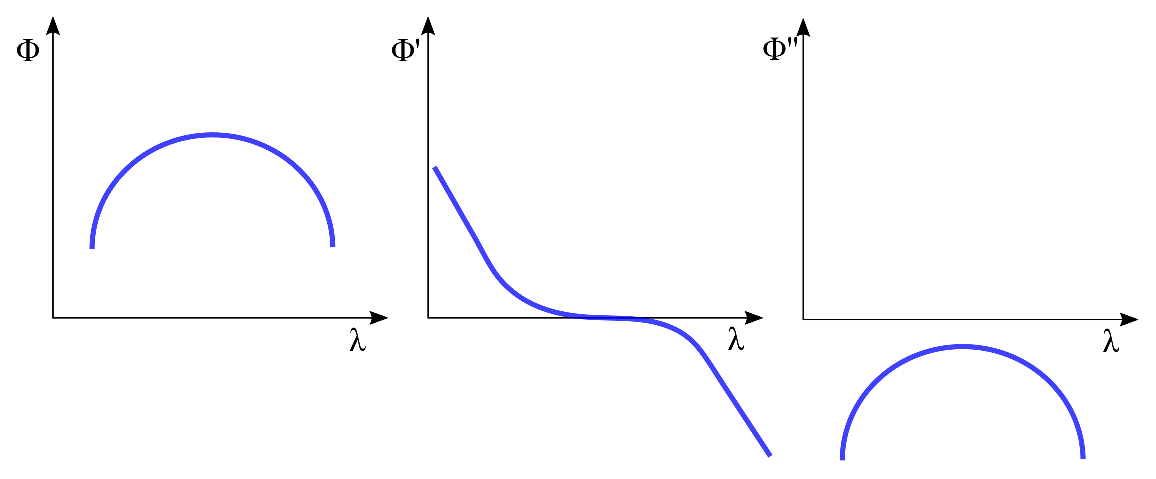
\includegraphics[scale=0.6]{PhiConvex}
    \caption[Connection one to one between $\lambda$ and $a$]{Representation of the convex functional $\Phi[\lambda]$ and its first and second derivative.}
    \label{fig:PhiConvex}
\end{figure}

This argument is  valid for  any pair  of conjugate variables  and it
only depends on  the definition of the  conjugate variables introduced
in Eq. (\ref{relens1}).  It constitutes  the basic content of the DFT
when the relevant variable is the microscopic density operator.

Because the  connection is one  to one,  we may change  variables from
$\lambda$ to $a$.   However, the average $a$ is given  by a derivative
and such a  change of variables implies a loss  of information.  As we
know from the usual treatment in Thermodynamics \cite{Callen1960}, the
correct way to proceed is to  introduce the dimensionless entropy function $S[a]$ of
the given  level of description  as the (minus) Legendre  transform of
the thermodynamic potential in the form
\begin{align}
S[a] &=-\Phi[\lambda[a]]+\lambda[a] a
\label{entropya}\end{align}
The  relation of  this entropy  function $S[a]$  and the  Gibbs-Jaynes
entropy functional  ${\cal S}[\overline{\rho}]$ in  (\ref{entropy}) is
simple. The  former is just  the later  evaluated at its  maximum, the
relevant ensemble (\ref{relens1}). This is
\begin{align}
S[a]={\cal  S}[\overline{\rho}]
\end{align}
Because  the  entropy   $S[a]$  is  the  Legendre   transform  of  the
thermodynamic  potential  $\Phi[\lambda]$,  we have  the  relationship
conjugate to (\ref{cg1})
\begin{align}
  \frac{\partial S}{\partial a}&=\lambda
\label{e3}
\end{align}


\section{The dynamics}\label{sec:Grabert}
In general it is possible to derive the evolution equation for a given
dynamic  variable  by  using  the technique  of  projection  operators
\cite{Kawasaki1973a,Grabert1982}. The projection operator method can be
understood, at its most fundamental level  as a way to approximate the
actual time dependent ensemble, which is the solution of the Liouville
equation, with a relevant  ensemble of the form (\ref{relens1}),
plus  a correction,  which  is the  responsible  for the  irreversible
behaviour. We  summarize   in  the   rest  of   this  section   the
time-dependent  projection  operator  technique as  presented  in  the
classical  textbook  by Grabert  \cite{Grabert1982}.   

The  aim is  to
derive equations of motion for  the time dependent average $a_i(t)$ of
the set of relevant variables $\hat{A}_i(z)$. The time dependent average
is
\begin{equation}
  a_i(t)={\rm Tr}[\rho_t\hat{A}_i]
  \label{ave}
\end{equation}
where $\rho_t$ is
the non-equilibrium solution of the Liouville equation. As it is shown
in  \cite{Grabert1982},  for  isolated systems  with a time-independent
Hamiltonian,  the   averages  (\ref{ave})  evolve  according   to  the
following closed exact equation

\begin{equation}
\frac{\partial }{\partial t} a_i(t)
= v_i(t) + \int_0^t dt' \sum_j K_{ij}(t,t') \lambda_j(t')
\label{ex}
\end{equation}
The reversible term is given by
\begin{equation}
v_i(t) = {\rm Tr}[\overline{\rho}_t  iL \hat{A}_i]
\label{vit}
\end{equation}
where $iL$ is the Liouville operator (\ref{iL})

The  relevant
ensemble $\overline{\rho}_t$  is of  the form (\ref{relens1}),  with a
time   dependent  conjugate   variable  $\lambda(t)$.   The  conjugate
variables  $\lambda$ are  selected in  such  a way  that the  averages
$a(t)$ of the  real and of the relevant ensemble  coincide.  Note that
if   only  the   reversible  term   $v_i(t)$  would   be  present   in
Eq. (\ref{ex}), we would be  approximating the actual ensemble that it
is a  solution of the Liouville  equation with a relevant  ensemble of
the form (\ref{relens1}) where the conjugate field $\lambda(t)$ is now
a function of time.  The error  in this approximation is, in fact, the
memory term which describes  irreversible behaviour.  The irreversible
term in Eq. (\ref{ex}) involves the memory kernel
\begin{equation}
K_{ij}(t,t') =
{\rm Tr}[\overline{\rho}_{t'} 
\left({\cal Q}_{t'} iL\hat{A}_j\right) G_{t't}
\left({\cal Q}_{t } iL\hat{A}_i\right)]
\label{ker}
\end{equation}
where   the  Kawasaki-Gunton   projection  operator   ${\cal  Q}_{t'}$
\cite{Kawasaki1973a,  Grabert1982}  applied  to an  arbitrary  function
$\hat{F}(z)$ is
\begin{eqnarray}
{\cal Q}_{t'}\hat{F}(z)& = &\hat{F}(z)- {\rm Tr}[\overline{\rho}_{t'} \hat{F}]
\nonumber\\
&-&\sum_i(\hat{A}_i(z)-a_i(t'))\frac{\partial }{\partial a_i(t')}
{\rm Tr}[\overline{\rho}_{t'} \hat{F}]
\label{Q}
\end{eqnarray}
Finally, the time ordered projected propagator $G_{t't}$ is given by formal series
\begin{eqnarray}
G_{t't}&=&1
+\sum_{n=1}^\infty \int_{t'}^tdt_1\cdots\int_{t'}^{t_{n-1}}dt_n
 iL{\cal Q}_{t_n}\cdots  iL{\cal Q}_{t_1}
\nonumber\\
&=&T_-\exp\left\{\int_{t'}^t dt''  iL{\cal Q}_{t''}\right\}
\end{eqnarray}
Eq.   (\ref{ex}) is  a closed  exact equation  for the  time dependent
averages $a(t)$.  The only assumption  taken in deriving (\ref{ex}) is
that the initial  ensemble to be used in the  Liouville equation is of
the relevant form.  This is, it is assumed that  the only knowledge at
the initial  time is the value  of the average $a(0)$  and, therefore,
the  least   biased  initial   ensemble  is   of  the   relevant  form
(\ref{relens1}).  Therefore, the time  dependent average $a(t)$ of the
relevant variables $\hat{A}(z)$  is computed with the  solution of the
Liouville equation $\rho_t(z)$  with an initial condition  which is of
the relevant  form.  The relevant  ensemble is a functional  of $a(t)$
through  $\lambda(t)$.   The kernel  becomes  a  functional of  $a(t)$
through the relevant  ensemble.  

Although Eq.  (\ref{ex})  is a closed
equation it is an integro-differential  equation which is difficult to
treat  in   general.   Nevertheless,  the  exact   transport  equation
(\ref{ex}) can  be approximated by  a memory-less equation  whenever a
clear separation  of time scales  exists between the evolution  of the
averages and  the decay of  the memory kernel. Under  this assumption
and the  neglect of terms of  order ${\cal O}( iL\hat{A}^3)$,  assumed to be
small due to  the slowness of the relevant variables,  one obtains the
Markovian equation \cite{Grabert1982}
\begin{equation}
\dot{a}_i(t) = v_i(t) + \sum_j D_{ij}(t) \lambda_j(t)
\label{ex2}
\end{equation}
where  the  dissipative matrix  is  given  by  the Green-Kubo  formula
\begin{equation}
D_{ij}(t)=\int_0^{\Delta t} dt'\left\langle 
{\cal Q}_t iL\hat{A}_j\exp\{iLt'\}{\cal Q}_t iL\hat{A}_i
\right\rangle^{\lambda(t)}
\label{dij}
\end{equation}
Here,  $\Delta t$ is  a  time large  compared  to the  decay  time of  the
correlation  integrand  but  short  in  front of  the  time  scale  of
evolution of  the relevant variables.  The  dissipative matrix depends
in general  on the  relevant variables  through the  relevant ensemble
and, as such, it is a function of time.  The dissipative matrix is, to
the  extent that  the  Markov property  holds,  positive definite  and
satisfies Onsager's reciprocity \cite{Grabert1982}.

It is straightforward  to show that the  dynamic equations (\ref{ex2})
have  as  a  Lyapunov   function  the  entropy  (\ref{entropya})  and,
therefore,   the   dynamics   complies   with  the   Second   Law   of
Thermodynamics.  The  equations (\ref{ex2})  predict the decay  of any
initial value  of the  average of the  relevant variables  towards its
unique equilibrium  values. Forced situations may  be treated
with the present  formalism \cite{Grabert1982} but we  do not consider
them here for simplicity.


\section{Summary}



%CHAPTER 2
\chapter{Continuous hydrodynamics theory for liquids near solids}\label{Chap:Theory}
\markboth{Continuous hydrodynamics theory for liquids near solids}{}
\epigraph{\textit{Le temps est une invention du mouvement. Celui qui ne bouge pas ne voit pas le temps passer.}}{Métaphysique des tubes \\ AMÉLIE NOTHOMB}
\section{Introduction}

\section{The system and the relevant variables}
In this section we use the ToCG described in the previous chapter for describing hydrodynamically a liquid near a solid. 
Consider a liquid system of $N$ monoatomic molecules described
with the position and momenta of  their center of mass.  The molecules
are allowed to move through  space unrestrictedly. To avoid the issues
of  an infinite  number  of particles  required  in the  thermodynamic
limit, and to make closer contact with molecular dynamics simulations,
we simply  assume that  the system  has periodic  boundary conditions.
Interacting with that sea of liquid molecules there is a group of $N'$
bonded atoms forming  what we would understand at a macroscopic level
as a solid object of spherical shape. \Note{By considering the interaction of a liquid with a solid sphere, we may address the issue of total momentum conservation that may become rather obscure if one considers "planar walls with infinite mass".}
In addition, we take a solid sphere because then only the position and the momentum of the center of mass is required in order to have a coarse-grained description of the solid sphere. For non-spherical particles, it is necessary, in general, to include also the orientation  and angular velocity of the sphere, as this is expected to play an important role in the dynamics. 
Still, even in the spherical object case, it may be important to introduce angular velocity in order to have accurate results. 
However, for the sake of simplicity and presentation of the basic results, we restrict ourselves in this paper to the simplest case without angular variables for the solid sphere.  


At the microscopic level the system is described  by the set of
as this is expected to play an important role in the dynamics. Still, all  positions  ${\bf  q}_i$  and  momenta  ${\bf  p}_i=m_i{\bf  v}_i$
($i=1,\cdots,N$) of the liquid atoms plus the positions ${\bf q}_{i'}$
and  momenta ${\bf  p}_{i'}=m_{i'}{\bf v}_{i'}$  ($i'=1,\cdots,N'$) of
the atoms  of the solid  sphere.  For  compactness we will  denote the
microstate in either  of the following forms $z$  or ${q,p,q',p'}$. We
will distinguish  with a prime  the labels of  the atoms of  the solid
sphere from the  unprimed labels of the liquid  atoms.  The microstate
of  the  system  evolves  according to  Hamilton's  equations  with  a
Hamiltonian given by
\begin{eqnarray}
H(z) &=& \sum^N_i \frac{p_i^2}{2m_i} + \sum^{N'}_{i'} \frac{p_{i'}^2}{2m_{i'}}
+ U(z)
\label{H}
\end{eqnarray}
where the potential energy $U(z)$ is given by
\begin{align}
U(z)&=  V^{f}(q)+ V^{fs}(q,q')+ V^{s}(q')
\end{align}
We  assume   for  simplicity  a  pair-wise   potential  energy,  where
$V^{f}(q)=\frac{1}{2}\sum^{{NN}}_{i   j}\phi^{ll}_{ij}$   is   the
potential  of  interaction  between   liquid  atoms,  $  V^{ls}(q,q')=
\sum^{NN'}_{ii'}\phi^{ls}_{ii'}$  is  the   potential  of  interaction
between   liquid   atoms   and   solid   atoms,   and   $   V^{s}(q')=
\frac{1}{2}\sum^{{N'N'}}_{i' j'}\phi^{ss}_{i'j'}$ is the potential
of  interaction  between   the  atoms  of  the   solid  object.   Self
interaction of  the atoms  is not  considered, so  $\phi_{ii}=0$, etc.
There are  no external conservative  potentials acting on  the system,
although  they can  be  easily  introduced. We  do  not consider  such
external potentials  in order to  transparently discuss the  issues of
momentum conservation.

Note that at a microscopic level we do not have boundaries of
  any kind, we only have particles interacting with particles in free
(periodic) space.  In lab  situations, typically, liquids are contained
in flasks and other type of  solid objects that prevent the liquid from
leaking.  We could model a spherical  flask containing a liquid in very
much  the same  way  as we  are  going to  treat  the solid  spherical
particle  surrounded  by  the  (possibly  infinite  in  extension,  or
periodic)  liquid. A solid is
  regarded as a collection of  bounded atoms (that is, their relative
distances  do  not  increase  without   bound)  that  are  moving  and
vibrating. The spherical  shape of the particle  should be understood,
of course, in a statistical sense.

\subsection{The relevant variables}
We describe the system at a coarse grained level by selecting as
relevant variables the  mass and momentum density fields  of the liquid
and  the   center  of  mass   position  and  momentum  of   the  solid
sphere. These are given by the following set of phase functions 
\begin{align}
  \hat{\rho}_{\bf r}(z) &=\sum^{N}_im\delta({\bf r}-{\bf q}_i),
&&\hat{\bf R}(z)=\frac{1}{N'}\sum_{i'}^{N'}{\bf q}_{i'}
\nonumber\\
  \hat{\bf g}_{\bf r}(z) &=\sum^{N}_i{\bf p}_i\delta({\bf r}-{\bf q}_i),
&&\hat{\bf P}(z)=\sum_{i'}^{N'}{\bf p}_{i'}
\label{CGvar}
\end{align}
In these phase  functions, the position ${\bf r}$ plays  the role of a
continuous index labeling  the phase function. The  position ${\bf r}$
may take any value in  $\mathbb{R}^3$, or its periodic counterpart, as
we  do  not  have  any  restriction to  the  possible  motion  of  the
particles. The hamiltonian (\ref{H}) is also a relevant variable.

For the sake of simplicity, we do not include orientational degrees of
freedom of the  solid for the time being.  Note  that by selecting the
center of  mass variables of the  solid as the only  ones necessary to
describe the  state of the solid  we are implicitly assuming  that the
remaining  solid  degrees   of  freedom  are  much   faster  than  the
hydrodynamic  fields.   In  particular,  we assume  that  any  elastic
behaviour of the solid is  so rapidly decaying towards its equilibrium
state  that elastic  variables  do  not need  to  be  included in  the
description. Should this assumption be violated, the resulting dynamic
equations (not including  these elastic variables for the solid)
would probably  be non-Markovian.

A word is in order about a  model for the solid that is sometimes used
in  simulation work,  where the  solid  is  assumed to  be made  of
``frozen''  particles that  act  as simple  generators  of forces  not
reacting back  to the presence of  the liquid. In this  case, the solid
should be modeled as a static external field acting on the liquid. The
structure of the theory changes in this case as we will discuss later.

\subsection{The time derivatives of the relevant variables}
The time derivatives  of the coarse variables play  a fundamental role
in the final structure of  the dynamic equations (\ref{ex2}). The time
derivative $  iL\hat{A}$ is  the result of  applying the  Liouville operator
(\ref{iL}) to the relevant variables.  In this section, we discuss the
particular  form of  $  iL\hat{A}$ for  the case  of  selected CG  variables
(\ref{CGvar}). The action of the Liouville operator on the CG variables gives \cite{Espanol2015a}
\begin{eqnarray}
  iL \hat{\rho}_{\bf r}(z) &=& -\boldsymbol{\nabla}\esc\hat{\bf g}_{\bf r}(z)
\nonumber\\
iL  \hat{\bf g}_{\bf r}(z) &=& -\boldsymbol{\nabla}{\cdot} \hat{{\bf K}}_{\bf r}(z)+
\hat{\bf F}^l_{\bf r}(z)
\label{ildens}
\end{eqnarray}
Here, the kinetic stress tensor is 
\begin{align}
  \hat{{\bf K}}_{\bf r}(z) &=\sum^{N}_i{\bf p}_i{\bf v}_i
\delta({\bf r}-{\bf q}_i)
\end{align}
and the total force density $\hat{\bf F}^l_{\bf r}(z)$  on the liquid
is defined as
\begin{align}
  \hat{\bf F}^l_{\bf r}(z) &
=\sum_i^N-\frac{\partial U}{\partial {\bf q}_i}\delta({\bf r}-{\bf q}_i)
\label{Frtot}
\end{align}
We may decompose  this force density into the
force that  the liquid exerts on  the liquid plus the  force that the
solid   exerts  on  the   liquid,  this   is,  
\begin{align}
   \hat{\bf  F}^l_{\bf
  r}(z)&=\hat{\bf  F}^{\rm l\to  l}_{\bf r}(z)  +\hat{\bf  F}^{\rm s\to
  l}_{\bf r}(z) 
\nonumber\\
\hat{\bf F}^{\rm l\to l}_{\bf r}(z) &= \sum^{NN}_{ij}\hat{\bf F}_{ij}\delta({\bf r}-{\bf q}_i)
\nonumber\\
\hat{\bf F}^{\rm s\to l}_{\bf r}(z) &= \sum^{NN'}_{ij'}\hat{\bf F}_{ij'}\delta({\bf r}-{\bf q}_i)
\label{Fr}
\end{align}
where $\hat{\bf F}_{ij'}$ is the force  that atom $j'$ of the solid
exerts on  atom $i$ of  the liquid.   This is, $\hat{\bf  F}^{\rm l\to
  l}_{\bf r}(z)  $ is  the microscopic force  density that  the liquid
exerts on the liquid molecules that are around the point ${\bf r}$ and
$\hat{\bf F}^{\rm s\to l}_{\bf r}(z)$ is the microscopic force density
that the solid object exerts on the liquid at the point ${\bf r}$.

We may write the force that the liquid exerts on te liquid 
\begin{align}
  \hat{\bf F}^{\rm l\to l}_{\bf r}(z) &= \frac{1}{2}\sum^{NN}_{ij}\hat{\bf F}_{ij}
(\delta({\bf r}-{\bf q}_i)-\delta({\bf r}-{\bf q}_j))
\end{align}
where we  have used that  the indices are  dummy. By using  a standard
trick \cite{Schofield1982,Grabert1982}, we  may express the difference
of the Dirac delta functions in terms of a divergence
\begin{align}
\delta({\bf r}-{\bf q}_i)-\delta({\bf r}-{\bf q}_j)
=&\int_0^1d\epsilon\frac{d}{d\epsilon}
\delta({\bf r}-{\bf q}_j-\epsilon{\bf q}_{ij})
\nonumber\\
=&-\nabla\int_0^1d\epsilon{\bf q}_{ij}
    \delta({\bf r}-{\bf q}_j\Note{-\epsilon{\bf q}_{ij}})
\nonumber\\
\label{trick}
\end{align}
\Note{Aclarar si es $-\epsilon q_{ij}$ o $\epsilon q_{ij}$.}

The liquid  force density  $\hat{\bf F}^{\rm  l\to l}_{\bf  r}(z)$ can
then be expressed  as the divergence of the  microscopic virial stress
tensor, this is
\begin{align}
\hat{\bf F}^{\rm l\to l}_{\bf r}(z)&=-\boldsymbol{\nabla}\cdot \hat{\boldsymbol{\Pi}}_{\bf r}(z)
\nonumber\\
\hat{\boldsymbol{\Pi}}_{\bf r}(z)&\equiv \frac{1}{2}\sum^{N}_{ij}{\bf q}_{ij}\hat{\bf F}_{ij}
\int_0^{1}d\epsilon\delta({\bf r}-{\bf q}_i-\epsilon{\bf q}_{ij})
\label{micfluxes}
\end{align}
The time derivative of the momentum density (\ref{ildens}) becomes
\begin{align}
    iL\hat{\bf g}_{\bf r}(z)
    &=-\boldsymbol{\nabla}\cdot \hat{{\bf K}}_{\bf r}(z) - \boldsymbol{\nabla}\cdot \hat{{\bf     \Pi}}_{\bf r}(z) +  {\bf F}^{\rm s\to l}_{\bf r}(z) \nonumber \\
    &= -\boldsymbol{\nabla}\cdot\left(\hat{{\bf K}}_{\bf r}(z)+\hat{{\bf \Pi}}_{\bf r}(z)\right) +{\bf F}^{\rm s\to l}_{\bf r} \nonumber \\
    &=-\boldsymbol{\nabla}\cdot \hat{\boldsymbol{\sigma}}_{\bf r}+{\bf F}^{\rm s\to l}_{\bf r},
\label{gls}
\end{align}
where     $\hat{\boldsymbol{\sigma}}_{\bf r}(z)=\hat{{\bf K}}_{\bf
r}(z)+\hat{\boldsymbol{\Pi}}_{\bf r}(z)$  is the microscopic stress
tensor of the fluid, this is
\begin{align}
  \hat{\boldsymbol{\sigma}}_{\bf r}(z)=&
\sum^{N}_i{\bf p}_i{\bf v}_i
\delta({\bf r}-{\bf q}_i)\nonumber\\
&+
\frac{1}{2}\sum^{N}_{ij}{\bf q}_{ij}\hat{\bf F}_{ij}
\int_0^{1}d\epsilon\delta({\bf r}-{\bf q}_i-\epsilon{\bf q}_{ij})
\label{sigma}
\end{align}

For the solid object we have that the action of the Liouville operator gives
\begin{align}
    iL\hat{\bf R}(z) &=\frac{\hat{\bf P}(z)}{M}
  \nonumber\\
    iL\hat{\bf P}(z) &=-\int  d{\bf r} \hat{\bf F}^{\rm s\to l}_{\bf r}(z)
   \label{Pfsl}  
\end{align} 

Note  that the  total  momentum,  which is  defined  in  terms of  the
coarse-grained variables as
\begin{align}
  \hat{\bf P}_T&=\int d{\bf r} \hat{\bf g}_{\bf r}(z)+\hat{\bf P}(z)
\end{align}
satisfies $ iL\hat{\bf P}_T=0$ and is, therefore, a conserved quantity
of  the  microscopic   dynamics.   We  have  used   that  $\int  d{\bf
  r}\boldsymbol{\nabla}\esc\hat{\boldsymbol{\sigma}}=0$  due to  Gauss theorem  and the  fact
that at the infinite we assume there are no fluid molecules. A similar
argument holds when the domain of integration is periodic.


Summarizing, the time derivatives of the relevant variables of the system are
\begin{align}
    iL \hat{\rho}_{\bf r}(z) &= -\boldsymbol{\nabla}\esc\hat{\bf g}_{\bf r}(z)
\nonumber\\
iL\hat{\bf g}_{\bf r}(z)
&=-\boldsymbol{\nabla}\cdot \hat{\boldsymbol{\sigma}}_{\bf r}(z)+{\bf F}^{\rm s\to l}_{\bf r}(z) \nonumber \\
    iL\hat{\bf R}(z) &=\frac{\hat{\bf P}(z)}{M}
  \nonumber\\
    iL\hat{\bf P}(z) &=-\int  d{\bf r} \hat{\bf F}^{\rm s\to l}_{\bf r}(z)
   \label{timeDerivatives}  
\end{align}

\section{The relevant ensemble and the grand potential}
In section \ref{sec:TheEntropy} we obtained that the ensemble which maximizes the Gibbs-Jaynes entropy function (\ref{entropy}) is of the type
\begin{equation}
\overline{\rho}(z) = \frac{1}{Z[\lambda]} \rho_0\exp\{-\lambda\!\cdot\!\hat{A}(z)\}
%\label{relens1}
\end{equation}
When the CG variables are those in (\ref{CGvar}), the relevant ensemble $\bar{\rho}(z)$ takes the form
\begin{eqnarray}
  \overline{\rho}(z)&=&\frac{1}{\Xi[\lambda]}\rho_0\exp\left\{-\beta H_N(z)\right\}
\nonumber\\
&\times&
\exp\left\{-\beta\int d{\bf r}\left(\lambda_\rho({\bf r})\hat{\rho}_{\bf
    r}(z)+\boldsymbol{\lambda}_g{({\bf r})\cdot}\hat{\bf g}_{\bf r}(z)\right)\right\}
\nonumber\\
&\times&
\exp\left\{-\beta \boldsymbol{\lambda}_{R}\esc\hat{\bf R}(z)
-\beta \boldsymbol{\lambda}_{P}\esc\hat{\bf P}(z)\right\}
\nonumber\\
\label{relensln}
\end{eqnarray}
The   normalization   factor   is  the   $\lambda$-dependent
grand-canonical partition function defined as
\begin{align}
&\Xi[\lambda]
\equiv
 \sum_{N=0}^\infty \frac{1}{N!h^{3N}}
\int dqdp dq'dp'
\nonumber\\
&\times\exp\left\{-\beta H_N(z)-\beta \sum_{i=1}^Nm\lambda_\rho({\bf
    r}_i)-\beta \sum_{i=1}^N{\bf p}_i\esc\boldsymbol{\lambda}_g({\bf q}_i)\right\}
\nonumber\\
&\times\exp\left\{-\beta \boldsymbol{\lambda}_{R}\esc\hat{\bf R}(z)
-\beta \boldsymbol{\lambda}_{P}\esc\hat{\bf P}(z)\right\}
\label{xiln}
\end{align}
The conjugate fields $\lambda$ of the CG variables (\ref{CGvar}) are fixed by the condition that the averages of the CG variables with the relevant ensemble coincide with the averages $\rho({\bf  r}),{\bf  g}({\bf
  r}),{\bf  R},{\bf  P}$  computed  with  the 
  solution of  the Liouville equation (we omit the time  dependence for simplicity). This conditions can be expressed as in Eqs. (\ref{cg1}) 
\begin{align}
  \rho({\bf r}) &=\frac{\delta \Phi [\lambda]}{\delta \lambda_\rho({\bf r}) }
&&{\bf R} =\frac{\partial \Phi [\lambda]}{\partial \boldsymbol{\lambda}_R }
\nonumber\\
  {\bf g}({\bf r}) &=\frac{\delta \Phi [\lambda]}{\delta \boldsymbol{\lambda}_g({\bf r}) }
&&{\bf P} =\frac{\partial \Phi [\lambda]}{\partial \boldsymbol{\lambda}_P }
\label{rgo}
\end{align}
where the $\lambda$-dependent grand-canonical potential is given, as in Eq. (\ref{PhiLambda}) by
\begin{eqnarray}
  \Phi [\lambda]&\equiv&-k_BT \ln\Xi [\lambda]
\label{oh}
\end{eqnarray}
As we saw in section (\ref{sec:TheEntropy}), there is a one to one connection between the CG variables and the conjugate ones becasuse the functional $\Phi[\lambda]$ is convex.  
Therefore, the  functionals $\lambda_{\rho}[\rho,{\bf  g},{\bf R},{\bf
  P}]$,   $\boldsymbol{\lambda}_g[\rho,{\bf   g},{\bf  R},{\bf   P}]$,
$\boldsymbol{\lambda}_R[\rho,{\bf      g},{\bf      R},{\bf      P}]$,
$\boldsymbol{\lambda}_P[\rho,{\bf g},{\bf  R},{\bf P}]$ exist  and are
unique.   We  can  therefore   switch  from  the  conjugate  variables
$\lambda$   to  the   relevant   variables  $a$   and  construct   the
corresponding hydrodynamic functional.The   hydrodynamic functional   is    given   by   the   Legendre    transform   of   the $\lambda$-dependent grand canonical potential, this is
\begin{align}
{\cal H}[\rho,{\bf g},{\bf R},{\bf P}] &=
\Phi [\lambda_\rho,\boldsymbol{\lambda}_g,\boldsymbol{\lambda}_R,\boldsymbol{\lambda}_P]
\nonumber\\
& -
\int d{\bf r}\rho({\bf r})\lambda_\rho({\bf r})
-
\int d{\bf r}{\bf g}({\bf r})\cdot\boldsymbol{\lambda}_g({\bf r})
\nonumber\\
&
-\boldsymbol{\lambda}_R\cdot{\bf R}-\boldsymbol{\lambda}_P\cdot{\bf P}
\label{oleg}
\end{align}

Note that the hydrodynamic functional  is the negative of the corresponding entropy (\ref{entropya}) for the present level of description. Therefore, the Eq. (\ref{e3}) must be satisfied.

\begin{align}
  \lambda_\rho({\bf r}) &=-\frac{\delta {\cal H}}{\delta \rho({\bf r}) }
&&  \boldsymbol{\lambda}_R =-\frac{\partial {\cal H}}{\partial {\bf R} }
\nonumber\\
  \boldsymbol{\lambda}_g({\bf r}) &=-\frac{\delta {\cal H}}{\delta {\bf g}({\bf r}) }
&&  \boldsymbol{\lambda}_P =-\frac{\partial {\cal H}}{\partial{\bf P} }
\label{lno}
\end{align}

It is possible to find the explicit expression of $\lambda_{\rho}({\bf r})$ and $\boldsymbol{\lambda}_g({\bf r})$ by performing the momentum integrals in Eq. (\ref{xiln}). Replacing in Eq. (\ref{xiln}) the Hamiltonian (\ref{H}) and the momentum of the solid (\ref{CGvar}) we obtain 
\begin{align}
\Xi[\lambda]
&\equiv
\sum_{N=0}^\infty \frac{1}{N!h^{3N}}
\int dqdpdq'dp'
\nonumber \\
&\times\exp\left\{-\beta U(z)-\beta \sum_{i=1}^Nm\lambda_\rho({\bf
    r}_i) -\beta \boldsymbol{\lambda}_{R}\esc\hat{\bf R}(z) \right\}
\nonumber \\
&\times
\exp\left\{-\beta \left(\sum_{i=1}^N\frac{{\bf p}_i^2}{2m_i} + \sum_{i=1}^{N'}\frac{{\bf p}_{i'}^2}{2m_{i'}} \right) - \beta \sum_{i=1}^N{\bf p}_i\esc\boldsymbol{\lambda}_g({\bf q}_i) 
-\beta \boldsymbol{\lambda}_P\sum_{i=1}^{N'}{\bf p}_{i'}\right\}
\end{align}
We may group the terms in this way
\begin{align}
\Xi[\lambda]
&\equiv
\sum_{N=0}^\infty \frac{1}{N!h^{3N}}
\int dqdpdq'dp'
\nonumber \\
&\times\exp\left\{-\beta U(z)-\beta \sum_{i=1}^Nm\lambda_\rho({\bf
    r}_i) -\beta \boldsymbol{\lambda}_{R}\esc\hat{\bf R}(z) \right\}
\nonumber \\
&\times
\exp\left\{-\beta \sum_{i=1}^N\left(\frac{{\bf p}_i^2}{2m_i} + {\bf p}_i\esc\boldsymbol{\lambda}_g({\bf q}_i)\right)\right\}
\exp\left\{-\beta \sum_{i=1}^{N'}\left(\frac{{\bf p}_{i'}^2}{2m_{i'}} + \boldsymbol{\lambda}_P{\bf p}_{i'}\right) \right\}
\end{align}
We perform the Gaussian integrals over momenta by using 
\begin{align}
\int_{-\infty}^{\infty} dx e^{-ax^2+bx}=\sqrt{\frac{\pi}{a}}e^{b^2/4a} 
\end{align}
reaching the following expression 
\begin{eqnarray}
\Xi [\lambda]
&\equiv&
 \sum_{N=0}^\infty \frac{1}{N!}
\int \frac{dq}{\Lambda^{3N}}\frac{dq'}{\Lambda^{3N'}}e^{-\beta U}
\nonumber\\
&\times&\exp\left\{-\beta \sum_{i=1}^N\left(m\lambda_\rho({\bf
    r}_i)-\frac{m}{2}\boldsymbol{\lambda}_{g}^2({\bf q}_i)\right)\right\}
\nonumber\\
&\times&\exp\left\{-\beta \left(\boldsymbol{\lambda}_R\cdot\hat{\bf R}-\frac{M'}{2}\boldsymbol{\lambda}_{P}^2\right)\right\},
\label{xiln2}
\end{eqnarray}
where we have introduced the thermal wavelength 
\begin{align}
\Lambda=\left(\frac{h^2\beta}{2\pi m}\right)^{\frac{1}{2}}
\end{align}
Together with Eq. (\ref{rgo}) and Eq. (\ref{oh})
\begin{align}
  \rho({\bf r}) &=\frac{\delta \Phi [\lambda]}{\delta \lambda_\rho({\bf r}) } = \frac{1}{\Xi[\lambda]} \frac{\delta\Xi [\lambda]}{\delta \lambda_{\rho}({\bf r})} = m
  \nonumber\\
  {\bf g}({\bf r}) &=\frac{\delta \Phi [\lambda]}{\delta \boldsymbol{\lambda}_g({\bf r}) } =\frac{1}{\Xi[\lambda]} \frac{\delta\Xi [\lambda]}{\delta \boldsymbol{\lambda_g}({\bf r})} = -m\cdot\boldsymbol{\lambda}_g({\bf r})
 \nonumber\\
  {\bf P} &=\frac{\partial \Phi [\lambda]}{\partial \lambda_P} =\frac{1}{\Xi[\lambda]} \frac{\partial\Xi [\lambda]}{\partial \lambda_P} = -M'\cdot\lambda_P
\end{align}
This leads directly to the explicit form of the following conjugate variables
\begin{align}
 \boldsymbol{\lambda}_g({\bf r}) &= -\frac{{\bf g}({\bf r})}{\rho({\bf r})}=-{\bf v}({\bf r})
\nonumber\\
 \boldsymbol{\lambda}_P &= -\frac{{\bf P}}{M'}
\label{nu}
\end{align}
and allows  one to interpret  these conjugate variables  as (negative)
velocities.  


We may express the gran potential (\ref{oh}) as a sum of two contributions
\begin{align}
\Phi [\lambda]&=  \Phi^{\rm pos}[\mu,\boldsymbol{\lambda}_R]
-\frac{M'}{2} {\boldsymbol{\lambda}_P}^2
\end{align}
where we have defined the following grand potential
\begin{align}
\Phi^{\rm pos}[\mu,\boldsymbol{\lambda}_R]
&\equiv-k_BT\ln
 \sum_{N=0}^\infty \frac{1}{N!}
\int \frac{dq}{\Lambda^{3N}}\frac{dq'}{\Lambda^{3N'}}\nonumber\\
&\times
\exp\left\{-\beta  \left(U-\sum_{i=1}^N m\cdot\mu({\bf
    r}_i)+ \boldsymbol{\lambda}_R\cdot\hat{\bf R}\right)\right\}
\label{xpos}
\end{align}
and the chemical potential per unit mass has been introduced as
\begin{align}
  \mu({\bf r})&\equiv\frac{1}{2}\lambda_g^2({\bf r})-\lambda_\rho({\bf r})
\label{chempot}
\end{align}

Note that the gran potential (\ref{xpos}) is similar to the macrocanonical gran potential of a fluid, except for the presence of the solid degrees of freedom and the corresponding conjugate variable $\boldsymbol{\lambda}_R$. 

\section{The free energy}
The Legendre transform of the gran potential for a simple liquid gives the classic (free energy) density functional and we may pursue the same route in order to define the free energy density functional of a fluid in the presence of a solid sphere. The Legendre transform of the gran potential (\ref{xpos}) is
\begin{align}
  {\cal F}[\rho,{\bf R}]&\equiv  \Phi^{\rm pos}[\mu,\boldsymbol{\lambda}_R]
-\mu({\bf r})\frac{\delta\Phi^{\rm pos}}{\delta\mu({\bf r})}[\mu,\boldsymbol{\lambda}_R] 
-\boldsymbol{\lambda}_R\frac{\partial \Phi^{\rm pos}}{\partial \lambda_R}[\mu,\boldsymbol{\lambda}_R] 
\label{legPrev}
\end{align}
The derivatives we need of the functional (\ref{xpos}) are \Note{(No me salen estas dos expresiones)}
\begin{align}
 \frac{\delta \Phi^{\rm pos}}{\delta \mu({\bf r})}[\mu,\boldsymbol{\lambda}_R]&=-
\langle \hat{\rho}_{\bf r}\rangle^{\mu,\boldsymbol{\lambda}_R}
\nonumber\\
  \frac{\partial \Phi^{\rm pos}}{\partial \boldsymbol{\lambda}_R}[\mu,\boldsymbol{\lambda}_R]&=
\langle \hat{\bf R}\rangle^{\mu,\boldsymbol{\lambda}_R}
\end{align}
where               the                averages               $\langle
\cdots\rangle^{\mu,\boldsymbol{\lambda}_R}$   are  defined   in  these
equations.  The second  derivatives of $ \Phi^{\rm pos}$  are given by
covariances  (see   Eqs.  (\ref{cg1})-(\ref{covariances}))   and  this
implies that $\Phi^{\rm  pos}[\mu,\boldsymbol{\lambda}_R]$ is a convex
function.  Therefore, the  connection between $\langle \hat{\rho}_{\bf
  r}\rangle^{\mu,\boldsymbol{\lambda}_R},       \langle       \hat{\bf
  R}\rangle^{\mu,\boldsymbol{\lambda}_R}$         and        $\mu({\bf
  r}),\boldsymbol{\lambda}_R$ is  one to  one. Note also  that because
the phase functions  $ \hat{\rho}_{\bf r}, \hat{\bf R}$  do not depend
on particle's momenta, we have that the averages are given by
\begin{align}
  \langle \hat{\rho}_{\bf r}\rangle^{\mu,\boldsymbol{\lambda}_R} &={\rm Tr}[\overline{\rho}\hat{\rho}_{\bf r}]=\rho_{\bf r}
\nonumber\\
  \langle \hat{\bf R}\rangle^{\mu,\boldsymbol{\lambda}_R} &={\rm Tr}[\overline{\rho}\hat{\bf R}]={\bf R}
\end{align}
Therefore,  we have  a one  to  one connection  between the  conjugate
variables  $\mu({\bf  r}),\boldsymbol{\lambda}_R$   and  the  averages
$\rho({\bf  r}),{\bf  R}$  of  the  CG  variables.


Finally, we have the free energy functional ${\cal  F}[\rho,{\bf R}]$ of a structured fluid in the presence of a solid sphere as the following Legendre transform
\begin{align}
  {\cal F}[\rho,{\bf R}]&\equiv  \Phi^{\rm pos}[\mu,\boldsymbol{\lambda}_R]
+
\int d{\bf r}\rho({\bf r})\mu({\bf r})-\boldsymbol{\lambda}_R\cdot{\bf R}
\label{leg}
\end{align}
whose derivatives are given by 
\begin{align}
   \frac{\delta {\cal F}}{\delta\rho({\bf r})}[\rho,{\bf R}] &=\mu({\bf r},{\bf R})
\nonumber\\
   \frac{\partial {\cal F}}{\partial{\bf R}}[\rho,{\bf R}] &=-\boldsymbol{\lambda}_R
\label{Fd2}
\end{align}
We can obtain an expression for the  hydrodynamic functional (\ref{oleg}) replacing the terms $\Phi[\lambda]$, $\boldsymbol{\lambda}_g({\bf r})$, $\boldsymbol{\lambda}_P$, and $\lambda_R\cdot{\bf R}$ by the Eqs. (\ref{xpos}), $(\ref{nu})$, and $(\ref{leg})$, respectively. 
\begin{align}
  {\cal H}[\rho,{\bf g},{\bf R},{\bf P}] =& 
  -\int d{\bf r} \rho({\bf r})\lambda_{\rho}({\bf r}) 
  +\int d{\bf r}\frac{{\bf g}^2({\bf r})}{\rho({\bf r})} 
  \nonumber\\
  &- {\cal F}[\rho,{\bf R}] -\int d{\bf r}\rho({\bf r})\mu({\bf r}) + \frac{{\bf P}^2}{2M'}
\end{align}
If we replace $\mu({\bf r})$ by the Eq. (\ref{chempot}) and use (\ref{nu}), we finally arrive to an expression of the hydrodynamic functional ${\cal H}$ which is the sum of a kinetic part and a "potential" part. 
\begin{align}
  {\cal H}[\rho,{\bf g},{\bf R},{\bf P}] &=   
  \underbrace{\int d{\bf r}\frac{{\bf g}^2({\bf r})}{2\rho({\bf r})} +\frac{{\bf P}^2}{2M'}}_{kinetic}
  +\underbrace{{\cal F}[\rho,{\bf R}]}_{\rm potential}
\label{oleg2}
\end{align}
\Pendiente{Desde ecuación (51) del paper hasta el final de la sección. En principio no veo que sea necesario añadirlo, pero me queda pensarlo detenidamente.}

\section{The transport equations}
In this section we will obtain the transport equation for a fluid in contact with a solid sphere. In section (\ref{sec:Grabert}) we obtained an expression for the evolution of the selected variables using the technique of projection operators which consists of an irreversible part and a reversible one. 
\subsection{Exact reversible dynamics}
In this subsection we consider the reversible part for the case that the CG variables are those in Eqs. (\ref{CGvar}).
For the mass density we have
\begin{align}
\left.\partial_t \rho({\bf r},t)\right|_{\rm rev}
&=  {\rm Tr}[\overline{\rho}_t  iL\hat{\rho}_{\bf r}] 
=-\boldsymbol{\nabla}\cdot {\bf  g}({\bf r},t)
\label{conrho}
\end{align}
where we have used Eq. (\ref{ildens}) and the fact that the relevant
ensemble average of $\hat{\bf g}_{\bf  r}$ is precisely  the momentum
density field ${\bf g}({\bf r},t)$.  On the other hand, and using again the Eq. (\ref{ildens}), the reversible
part of the momentum density evolution equation is
\begin{align}
\left.\partial_t {\bf g}({\bf r},t)\right|_{\rm rev}
&=  {\rm Tr}[\overline{\rho}_t  iL\hat{{\bf g}}_{\bf r}] 
\nonumber\\
&=-\boldsymbol{\nabla}\cdot  {\rm Tr}[\overline{\rho}_t \hat{{\bf K}}_{\bf r}] 
+  {\rm Tr}[\overline{\rho}_t  \hat{\bf F}^{\rm l}_{\bf r}]
\label{grev1}
\end{align}

We will compute the terms of Eq. (\ref{grev1}) taking advantage of the Galilean operator. 


The Galilean operator changes the velocity arguments from ${\bf v}_i\to {\bf v}_i-{\bf v}({\bf q}_i)$ for each $i$ fluid particle, this is
\begin{align}
&  {\cal G}\hat{F}({\bf q}_1,\cdots{\bf q}_N,{\bf p}_1,\cdots{\bf p}_N)
\nonumber\\
=&\hat{F}({\bf q}_1,\cdots{\bf q}_N,{\bf p}_1+m_1{\bf v}({\bf q}_1),\cdots{\bf p}_N+m_N{\bf v}({\bf q}_N))
\end{align}
The intuitive meaning of the Galilean operator is that when applied to a phase function gives how it is seen in a reference frame that moves with the flow field. \Note{Entender bien la forma intuitiva}. Within any trace this is just a change of variables. Therefore, we have the property
\begin{align}
  {\rm Tr}[\bar{\rho}_t\hat{F}] &= {\rm Tr}[({\cal G}\bar{\rho}_t)({\cal G}\hat{F})] \nonumber \\
  \label{Gprop}
\end{align}
The action of the Galilean operator on the relevant variables is
\begin{align}
  {\cal G}\hat{\rho}_{\bf r} &= \hat{\rho}_{\bf r} \nonumber\\
  {\cal G}\hat{g}_{\bf r} &= \hat{g}_{\bf r} + {\bf v}({\bf r})\hat{\rho}_{\bf r} \nonumber \\
  {\cal G}\hat{R}(z) &= \hat{R}(z) \nonumber\\
  {\cal G}\hat{P}(z) &= \hat{P}(z)
\end{align}
Therefore, the action of ${\cal G}$ on the relevant ensemble is \Note{(En el paper aparece $\rho^{eq}$ y no sé de dónde sale...)}
\begin{align}
  {\cal G}\overline{\rho}_t &=
\frac{1}{\Xi[\lambda(t)]}\rho_0
\exp\left\{\beta\int d{\bf r}\mu({\bf r})\hat{\rho}_{\bf r}(z)\right\}
\nonumber\\
&\times
\exp\left\{-\beta \boldsymbol{\lambda}_{R}(t)\esc\hat{\bf R}
-\beta \boldsymbol{\lambda}_{P}(t)\esc\hat{\bf P}\right\}
\label{resrelens}
\end{align}
where  the chemical  potential per  unit mass  has been  introduced in
Eq.  (\ref{chempot}).  \Note{Esta expresión de la colectividad relevante es gaussiana en momento pero el último término hace que sea lineal. ¿Por qué utilizamos el operador galileano si $\bar{\rho}_t$ sigue siendo gaussiana y con término lineal?}
The  action  of the  Galilean  operator on  the
microscopic kinetic stress tensor is
\begin{align}
  {\cal G}\hat{{\bf K}}_{\bf r} &=
\hat{{\bf K}}_{\bf r} 
+{\bf v}({\bf r})\hat{\bf g}_{\bf r}
+\hat{\bf g}_{\bf r}{\bf v}({\bf r})
+{\bf v}({\bf r}){\bf v}({\bf r})\hat{\rho}_{\bf r}
\end{align}
Using (\ref{Gprop}) we have
\begin{align}
  {\rm Tr}[\bar{\rho}_t\hat{{\bf K}}]={\rm Tr}[({\cal G}\bar{\rho}_t)({\cal G}\hat{{\bf K}}_{\bf r})]
\end{align}

By noting that the ensemble (\ref{resrelens}) is Gaussian in momenta, we have finally \Note{No consigo llegar a la siguiente expresión}
\begin{align}
  {\rm Tr}[\overline{\rho}_t \hat{{\bf K}}_{\bf r}] &=
{\bf v}({\bf r}){\bf v}({\bf r}){\rho}({\bf r})+\frac{k_BT}{m}\rho({\bf r})\boldsymbol{\delta}
\label{api}
\end{align}
where $\boldsymbol{\delta}$ is the unit  tensor.  

Now, let us consider the average of the total force density on the liquid, Eq. (\ref{Frtot})
\begin{align}
{\bf F}^l_{\bf r} &\equiv{\rm Tr}[\overline{\rho}_t \hat{\bf F}^l_{\bf r}] =
 \langle \hat{\bf F}^l_{\bf r}\rangle^{\mu,\boldsymbol{\lambda}_R}
\nonumber\\
&=
\frac{1}{\Xi[\mu,\boldsymbol{\lambda}_R]}
 \sum_{N=0}^\infty \frac{1}{N!}
\int \frac{dq}{\Lambda^{3N}}\frac{dq'}{\Lambda^{3N'}}
\left[\sum^{N}_{j}-\frac{\partial U}{\partial {\bf q}_{j}}\delta({\bf r}-{\bf q}_j)\right]
e^{-\beta U}
\nonumber\\
&\times \exp\left\{-\beta  \left( \boldsymbol{\lambda}_R\cdot\hat{\bf R}
-\sum_{i=1}^N m\mu({\bf q}_i)\right)\right\}
\end{align}
where we have  used the definition of the average  with respect to the
relevant ensemble,  after performing the momentum  integrals. Next, we
realize that the  derivative of the Boltzmann factor  is the potential
times the Boltzmann factor itself, this is
\begin{align}
{\bf F}^l_{\bf r}&=
\frac{1}{\Xi[\mu,\boldsymbol{\lambda}_R]}
 \sum_{N=0}^\infty \frac{1}{N!}
\int \frac{dq}{\Lambda^{3N}}\frac{dq'}{\Lambda^{3N'}}
\exp\left\{-\beta  \left(\boldsymbol{\lambda}_R\cdot\hat{\bf R}
-\sum_{i=1}^N m\mu({\bf   r}_i)\right)\right\}
\nonumber\\
&\times k_BT\sum^{N}_{j}\delta({\bf r}-{\bf q}_j)\frac{\partial }{\partial {\bf q}_{j}}e^{-\beta U}
\end{align}
Integrate by parts to obtain
\begin{align}
{\bf F}^l_{\bf r}&=
\frac{1}{\Xi[\mu,\boldsymbol{\lambda}_R]}
 \sum_{N=0}^\infty \frac{1}{N!}
\int \frac{dq}{\Lambda^{3N}}\frac{dq'}{\Lambda^{3N'}}
e^{-\beta U}
k_BT\sum^{N}_{j}-\frac{\partial }{\partial {\bf q}_{j}}\left[\delta({\bf r}-{\bf q}_j)
\exp\left\{-\beta  \left( \boldsymbol{\lambda}_R\cdot\hat{\bf R}
-\sum_{i=1}^N m\mu({\bf q}_i)\right)\right\}\right]
\nonumber\\
&=
\frac{1}{\Xi[\mu,\boldsymbol{\lambda}_R]}
 \sum_{N=0}^\infty \frac{1}{N!}
\int \frac{dq}{\Lambda^{3N}}\frac{dq'}{\Lambda^{3N'}}
e^{-\beta U}
\sum^{N}_{j}\exp\left\{-\beta  \left( \boldsymbol{\lambda}_R\cdot\hat{\bf R}
-\sum_{i\neq j}^N m\mu({\bf   q}_j)\right)\right\}
\nonumber\\
&\times k_BT\left[-\frac{\partial }{\partial {\bf q}_{j}}\delta({\bf r}-{\bf q}_j)
\exp\left\{\beta   m\mu({\bf   q}_j)\right\}\right]
\nonumber\\
&=\frac{k_BT}{m}\boldsymbol{\nabla} \rho({\bf r})
-\rho({\bf r})\boldsymbol{\nabla}\mu({\bf r})
\label{fllr}
\end{align}

By  collecting (\ref{api})  and  (\ref{fllr})  into  the  momentum  density  equation (\ref{grev1}) we obtain
\begin{align}
\left.\partial_t {\bf g}({\bf r},t)\right|_{\rm rev} 
&=-\boldsymbol{\nabla}\cdot\left({\bf v}({\bf r},t)  {\bf g}({\bf r},t)  \right)
-\rho({\bf r})\boldsymbol{\nabla}
\frac{\delta {\cal F}}{\delta\rho({\bf r})}[\rho,{\bf R}]
\label{grev}
\end{align}

In order to obtain the dynamics of the solid variables, we need to compute the average of the total force on the solid ${\bf F}^s$. We may follow identical steps as the case of the total force on the fluid ${\bf F}^f$ and obtain
\begin{align}
{\bf F}^s&={\rm Tr}[\overline{\rho}_t \hat{\bf F}^s]=
 \langle \hat{\bf F}^s\rangle^{\mu,\boldsymbol{\lambda}_R} 
\nonumber\\
&=\frac{1}{\Xi[\mu,\boldsymbol{\lambda}_R]}
 \sum_{N=0}^\infty \frac{1}{N!}
\int \frac{dq}{\Lambda^{3N}}\frac{dq'}{\Lambda^{3N'}}
\left[-\sum^{N'}_{i'}\frac{\partial U}{\partial {\bf q}_{i'}}\right]
e^{-\beta U}
\exp\left\{-\beta  \left(\sum_{i=1}^N m\mu({\bf
    r}_i)+ \boldsymbol{\lambda}_R\cdot\hat{\bf R}\right)\right\}
\nonumber\\
&=
\frac{1}{\Xi[\mu,\boldsymbol{\lambda}_R]}
 \sum_{N=0}^\infty \frac{1}{N!}
\int \frac{dq}{\Lambda^{3N}}\frac{dq'}{\Lambda^{3N'}}
\exp\left\{-\beta  \left(\sum_{i=1}^N m\mu({\bf
    r}_i)+ \boldsymbol{\lambda}_R\cdot\hat{\bf R}\right)\right\}
k_BT\left[\sum^{N'}_{i'}\frac{\partial }{\partial {\bf q}_{i'}}\right]e^{-\beta U}
\nonumber\\
&=
\frac{1}{\Xi[\mu,\boldsymbol{\lambda}_R]}
 \sum_{N=0}^\infty \frac{1}{N!}
\int \frac{dq}{\Lambda^{3N}}\frac{dq'}{\Lambda^{3N'}}
e^{-\beta U}
k_BT\left[-\sum^{N'}_{i'}\frac{\partial }{\partial {\bf q}_{i'}}\right]\exp\left\{-\beta  \left(\sum_{i=1}^N m\mu({\bf
    r}_i)+ \boldsymbol{\lambda}_R\cdot\hat{\bf R}\right)\right\}
\nonumber\\
&=
\frac{1}{\Xi[\mu,\boldsymbol{\lambda}_R]}
 \sum_{N=0}^\infty \frac{1}{N!}
\int \frac{dq}{\Lambda^{3N}}\frac{dq'}{\Lambda^{3N'}}
e^{-\beta U}
\exp\left\{-\beta  \left(\sum_{i=1}^N m\mu({\bf
    r}_i)+ \boldsymbol{\lambda}_R\cdot\hat{\bf R}\right)\right\}
\left[\sum^{N'}_{i'}\frac{\partial }{\partial {\bf q}_{i'}}\right] \boldsymbol{\lambda}_R\cdot\hat{\bf R}
\nonumber\\
&=\boldsymbol{\lambda}_R
\label{lf}\end{align}
This  identity  allows  one  to  interpret  physically  the  Lagrange
multiplier $\boldsymbol{\lambda}_R$ as the  force on the solid sphere.
By  using (\ref{Fd2})  we obtain  that the  total force  on the  solid
sphere is due to the gradient of the free energy functional
\begin{align}
{\bf F}^s&=-\frac{\partial  {\cal F}}{\partial{\bf R}}[\rho,{\bf R}]
\label{Fls}
\end{align}

Therefore, the averages with the relevant ensemble of the solid object variables are
\begin{align}
{\rm Tr}[\overline{\rho}_t  iL\hat{\bf R}] 
&=\frac{\bf P}{M}
\nonumber\\
{\rm Tr}[\overline{\rho}_t  iL\hat{\bf P}] 
&=-\frac{\partial {\cal F}}{\partial {\bf R}}[\rho,{\bf R}]
\end{align}
where we have used the Eq. (\ref{Fls}).

By collecting the  above results, the reversible part  of the dynamics
has the form
\begin{align}
\left.  \partial_t\rho({\bf r})\right|_{\rm rev}&=-\boldsymbol{\nabla}\cdot{\bf g}({\bf r})
\nonumber\\
\left.  \partial_t{\bf g}({\bf r})\right|_{\rm rev}&=-\boldsymbol{\nabla}\cdot\left({\bf g}({\bf r}){\bf v}({\bf r})\right)
-\rho({\bf r})\boldsymbol{\nabla} \frac{\delta {\cal F}}{\delta\rho({\bf r})}[\rho,{\bf R}]
\nonumber\\
\partial_t\left. {\bf R}\right|_{\rm rev}&=\frac{\bf P}{M}
\nonumber\\
\partial_t\left.{\bf P}\right|_{\rm rev}&=-\frac{\partial {\cal F}}{\partial {\bf R}}[\rho,{\bf R}]
\label{rev}
\end{align}
These reversible  equations are exact  as no approximations  have been
made so far. We qualify these  equations as reversible because, as can
be  explicitly  shown,  they   conserve  the  hydrodynamic  functional
(\ref{oleg}), which  is minus the entropy corresponding
  to this level of description.

\subsection{Markovian irreversible dynamics}
While the  reversible part of  the dynamics (\ref{rev}) is  exact, the
irreversible  part  that we  consider  is  approximate
because  we will  assume a  Markovian dynamics.   Under the  Markovian
approximation in which the memory kernel is assumed to decay in a time
scale  short  as compared  to  the  time  scales of  the  hydrodynamic
variables,   the  irreversible   dynamics   is  given   by  the   term
$\sum_jD_{ij}\lambda_j$   in  Eq.   (\ref{ex2}).   Because   the  time
derivatives of  $\rho({\bf r})$ and  ${\bf R}$  are given in  terms of
momenta, which  are relevant variables  themselves, the effect  of the
projection operator in (\ref{Q}) is simply ${\cal Q} iL\rho_{\bf r}=0$
and ${\cal Q}  iL{\bf R}_{\mu}=0$ resulting in  a large simplification
of  the  friction  matrix.   The irreversible  part  of  the  dynamics
$\sum_jD_{ij}\lambda_j$ in Eq. (\ref{ex2}) now takes the form
\begin{align}
\partial_t  \left(
    \begin{array}{c}
\rho({\bf r})\\
\\
{\bf g}({\bf r})\\
\\
{\bf R}\\
\\
{\bf P}
    \end{array}
\right)_{\rm irr}
&=
-\left(\begin{array}{cccc}
  0&0 &0&0\\
\\
0 &\int d{\bf r}'M^{gg}_{{\bf r}{\bf r}'}&0&M^{gP}_{\bf r}\\
\\
  0&0 &0&0\\
\\
0&\int d{\bf r}' M^{Pg}_{{\bf r}'}&0&M^{PP}
\end{array}\right)
\left(    \begin{array}{c}
\frac{\delta {\cal H}}{\delta \rho_{{\bf r}'}}\\
\\
\frac{\delta {\cal H}}{\delta {\bf g}_{{\bf r}'}}\\
\\
\frac{\partial {\cal H}}{\delta {\bf R}}\\
\\
\frac{\partial {\cal H}}{\delta {\bf P}}
    \end{array}
\right)
\label{irr1}
\end{align}
where we have  used (\ref{lno}). The sum over  the continuum ``index''
${\bf  r}$ becomes  an integral.   The domain  of integration  of this
integral  is  $\mathbb{R}^3$,  including  the interior  of  the  solid
sphere. By  using the  results (\ref{lno}),  (\ref{nu}) that  link the
functional derivatives of  the CG Hamiltonian with  respect to momenta
to the velocities, we obtain the following irreversible dynamics
\begin{align}
  \partial_t{\bf g}({\bf r})&=-\int d{\bf r}'M^{gg}_{{\bf r}{\bf r}'}
{\bf v}({\bf r}')-M^{gP}_{\bf r}{\bf V}
\nonumber\\
\frac{d}{dt}{\bf P}(t)&=-\int d{\bf r}' M^{Pg}_{{\bf r}'}{\bf v}({\bf r}')-M^{PP}{\bf V}
\label{IrrMark1}\end{align}
where the matrix elements are  defined in terms of Green-Kubo formulae
as
\begin{align}
  M^{gg}_{{\bf r}{\bf r}'}&=\frac{1}{k_BT}\int_0^{\Delta t} dt\langle 
{\cal Q}  iL\hat{\bf g}_{{\bf r}}(t){\cal Q}  iL\hat{\bf g}_{{\bf r}'}\rangle^\lambda
\nonumber\\
  M^{gP}_{{\bf r}}&=\frac{1}{k_BT}\int_0^{\Delta t} dt\langle 
{\cal Q}  iL\hat{\bf g}_{\bf r}(t){\cal Q}  iL\hat{\bf P}\rangle^\lambda
\nonumber\\
  M^{Pg}_{{\bf r}'}&=\frac{1}{k_BT}\int_0^{\Delta t} dt\langle 
{\cal Q}  iL\hat{\bf P}(t){\cal Q}  iL\hat{\bf g}_{{\bf r}'}\rangle^\lambda
\nonumber\\
  M^{PP}&=\frac{1}{k_BT}\int_0^{\Delta t} dt\langle 
{\cal Q}  iL\hat{\bf P}(t){\cal Q}  iL\hat{\bf P}\rangle^\lambda
\nonumber\\
\label{Ms}
\end{align}





\section{Summary}

%CHAPTER 3
\chapter{Boundary conditions}\label{Chap:BC}
\markboth{Boundary conditions}{}
\section{Introduction}
\section{Summary}

%CHAPTER 4
\chapter{Planar flows}\label{Chap:Planar}
\markboth{Planar flows}{}
\section{Introduction}
\section{Summary}

%CHAPTER 5
\chapter{Space and time locality of hydrodynamics in periodic boundary conditions}\label{Chap:PBC}
\markboth{Space and time locality of hydrodynamics in PBC}{}
\epigraph{\textit{Time is longer than any distance.}}{Absalom, Absalom! \\ WILLIAM FAULKNER}
\section{Introduction}



\section{Mori theory}
\label{Sec:Mori}
In this section we present a summary of Mori's theory in order to
set the notation and present a new Green-Kubo formula which avoid the plateau problem. 


At the more microscopic level of description we assume that the system is  well described  by classical  mechanics and  that the  microscopic state $z=\{{\bf q}_i,{\bf p}_i,i=1,\cdots,N\}$  is given by the set of positions  and momenta  of all  the atoms  in the  system.
At a macroscopic  level, we have  the system described with a  set of CG variables  that are phase functions arranged  into a column vector  $\hat{A}(z)$ with components $\hat{A}_\mu(z),\mu=1,\cdots,M$.   
The  corresponding  row  vector  is denoted  by  $\hat{A}^T$, where  $T$  stands  for transpose.   
Without loosing generality, we will assume that the equilibrium average of the CG variables  vanish.  
By  denoting by  $\hat{A}(t)=\hat{A}(z_t)$, the evolution of these functions in phase space is given by
\begin{eqnarray}
\frac{d}{dt}{\hat{A}}(t)=\exp\{i{\cal L}t\}i{\cal L}\hat{A}(z_0)
\label{LA}
\end{eqnarray}
Mori's  exact  Generalized Langevin  Equation  (GLE)  is an  evolution for the set of CG variables given by the following theorem
\begin{align}
\frac{d}{dt}\hat{A}(t) &= -L\esc C^{-1}(0)\esc \hat{A} (t)
-\int_0^tdt'\Gamma(t-t')\esc  C^{-1}(0)\esc \hat{A} (t') +F^+(t),
\label{exact}
\end{align}
where the following matrices have been introduced
\begin{eqnarray}
L&=&\langle \hat{A}i{\cal L}\hat{A}^T\rangle
\nonumber\\
C(0)&=&\langle \hat{A}\hat{A}^T\rangle
\nonumber\\
\Gamma(t)&=&\langle F^+(t)F^{+T}(0)\rangle,
\label{def}
\end{eqnarray}
where  $\langle\cdots \rangle$
denotes an equilibrium average
\begin{equation}
\langle\cdots\rangle\equiv \int dz\rho^{\rm eq}(z)\cdots,
\label{esc}
\end{equation}
and  $\rho^{eq}(z)$ is  the  equilibrium  ensemble.
The so called projected or random force is given by
\begin{align}
F^+(t)&= \exp\{{\cal Q}i{\cal L}t\} {\cal Q}i{\cal L}\hat{A}  
\label{Proj}
\end{align}
The projection operator ${\cal Q}$ is defined as ${\cal Q}=1-{\cal P}$
where  ${\cal P}$  is Mori's  projector whose  effect on  an arbitrary
phase function $\hat{F}(z)$ is
\begin{eqnarray}
  {\cal P}\hat{F}(z) &=& \langle \hat{F}\rangle+ \langle \hat{F}\hat{A}^T \rangle\esc  C^{-1}(0)\esc  \hat{A}(z)
\label{PM}
\end{eqnarray}
The  Mori  projector  (\ref{PM})   satisfies  that  ${\cal  P}\hat{A}=
\hat{A}$ and  transforms an arbitrary  function of phase space  into a
linear combination  of the  CG variables.   The projected  forces have
zero  mean  and  are  uncorrelated  from
previous values of the CG variables, this is 
\begin{align}
\langle  F^+  (t)\rangle&=0  
\nonumber\\
\langle \hat{A} F^+ (t)\rangle&=0 \quad\quad t\ge 0
\end{align}
We can introduce the matrix of correlations 
\begin{align}
  C(t)&=  \llangle \hat{A}(t)\hat{A}^T\rrangle
\end{align}
If we multiply the  exact equation (\ref{exact})  with $\hat{A}^T(z)$
and  average over  the equilibrium  ensemble, we  obtain a  closed and
exact equation for the correlation matrix of the CG variables
\begin{align}
  \frac{d}{dt}C(t)&=-L\esc C^{-1}(0)\esc C(t)
-\int_0^tdt' \Gamma(t-t')\esc C^{-1}(0)\esc  C(t')
\label{exactC}
\end{align}
Therefore, the GLE (\ref{exact}) allows  one to obtain not only an equation for the correlation of the CG variables, but also an equation for  their averages. 
If we multiply  (\ref{exact}) with an initial ensemble $\rho_0(z)$ and integrate over the microstates $z$ we obtain
\begin{align}
  \frac{d}{dt}a(t) &= -L\esc C^{-1}(0)\esc a(t)
  -\int_0^tdt' \Gamma(t-t')\esc  C^{-1}(0)\esc a(t')
\label{exactAve}
\end{align}
where the time-dependent average of the CG variables is defined as
\begin{align}
  a(t)&=\int dz \rho_0(z) \exp\{i{\cal L}t\}\hat{A}(z)
\end{align}
and we have assumed that the average of the random force with respect
to the initial ensemble vanishes, i.e.
\begin{align}
\int dz\rho_0(z)\exp\{{\cal Q}i{\cal L}t\} {\cal Q}i{\cal L}\hat{A}(z)=0
\label{F0}
\end{align}

\subsection{The Markovian approximation}
The Markovian approximation assumes that the CG variables evolve in a time scale much larger than the memory time scale. This implies that there exists  a time-independent matrix $M^*$
such that  the linear integro-differential term  in Eq. (\ref{exactC})
can  be  approximated  by  a  memory-less term,  also  linear  in  the
correlation matrix
\begin{align}
\int_0^tdt' \Gamma(t-t')\esc C^{-1}(0)\esc  C(t')&\simeq M^*\esc C^{-1}(0)\esc C(t)
\label{Markov1}
\end{align}
The  Markovian approximation  (\ref{Markov1})  in  the GLE  (\ref{exact})
implies the following evolution equation for the CG variables
\begin{align}
  \frac{d}{dt}\hat{A}(t) = -\Lambda^*\esc \hat{A} (t) +F^+(t),
\label{SDE}
\end{align}
where the dynamic matrix $\Lambda^*$ is defined as
\begin{align}
\Lambda^*\equiv(L+M^*)\esc C^{-1}(0)  
\label{Lambda}
\end{align}
The evolution of the average of the CG variables (\ref{exactAve}) under the Markovian approximation is
\begin{align}
  \frac{d}{dt}a(t) = -\Lambda^*\esc a(t)
\label{AproxAve}
\end{align}
And the evolution equation for the correlations (\ref{exactC}) takes the form  
\begin{align}
    \frac{d}{dt}C(t)&=-\Lambda^*\esc  C(t)
\label{AproxC}
\end{align}
This is  the evolution  equation of the  correlation matrix  under the
Markovian   approximation.    The   form   of   (\ref{AproxAve})   and
(\ref{AproxC}) illustrate Onsager's  regresion hypothesis, that states
that  (correlations  of) fluctuations   decay  as  the  averages.  Eqs
(\ref{AproxAve}), (\ref{AproxC}) show  that the transport coefficients
that appear in the transport equation for the averages are the same as
the  transport   coefficients  governing   the  correlations   of  the
fluctuations in equilibrium.


The solution of (\ref{AproxC})  is given by
the exponential matrix 
\begin{align}
  C(t)=\exp\{-\Lambda^* t\}\esc C(0)
\label{Csol}
\end{align}
This is  the main  prediction of  Mori theory that  states that  for a
linear Markovian theory  the only possibility for a  correlation is to
decay  in an  exponential  matrix  way. This  does  not  mean that  the
elements of  the correlation matrix  $C(t)$ decay as  $e^{-\alpha t}$,
because they are,  in fact, the sum of many  exponential terms that may
lead even to quasi-algebraic decays of correlations, as in the case of
hydrodynamics. 
%Los autovalores de la matriz C(t) decaen de forma exponencial, pero no los elementos de la matriz C(t). Estos, tal y como se observa en las gráficas de correlaciones se ajustan, en escala logarítmica, casi a una recta. Por eso tienen un comportamiento decayendo a cero casi-algebraico.

The Markovian Eq.  (\ref{AproxC})  cannot hold at
very short times,  because at $t=0$ the  exact equation (\ref{exactC})
implies
\begin{align}
    \frac{d}{dt}C(0)&=-L
\end{align}
which is only possible in  (\ref{AproxC}) if $M^*=0$. This paradoxical
result can  also be obtained  from Eq.  (\ref{Markov1}) because  if we
set $t=0$  in that  equation we obtain  again $M^*=0$.   Therefore, we
expect (\ref{AproxC}) to  hold  only after a time
$t=\tau$  larger than  the  decay of  the memory  kernel.  This is  an
important idea to keep in mind: correlations will decay in a Markovian
way only  after the time  beyond which memory  is lost. 
%The  value of
%$\tau$  should be  explicitly measured  in the  procedure to
%validate the Markovian approximation.

\subsection{The usual Green-Kubo formula is problematic}
In the previous section we have seen that the Markovian approximation assume that the memory kernel $\Gamma(t-t')$ decays in a typical molecular time scale in which $C(t')$ does not change appreciably. Therefore, we may approximate $C(t')\simeq C(t)$ within the memory integral, this is
\begin{align}
  \int_0^tdt' \Gamma(t-t')\esc c(t')&\simeq  \int_0^tdt' \Gamma(t-t')\esc  c(t)
\nonumber\\
&\equiv
M^+(t)\esc c(t)
\end{align}
where we have introduced the Green-Kubo running integral
\begin{align}
M^+(t)&\equiv  \int_0^tdt' \Gamma(t') 
\label{Mt}
\end{align}
and the normalized correlation matrix as
\begin{align}
  c(t)=C^{-1}(0)\esc C(t)
\end{align}
that at $t=0$ becomes the identity matrix.


For the Markovian approximation (\ref{Markov1}) to hold, we would need
that the matrix  $M^+(t)$ becomes time-independent.   Unfortunately,  the  matrix
$M^+(t)$ vanishes at $t=0$ and decays to zero at long times. In
fact,  the projected  force defined  in (\ref{Proj})  is a  total time
derivative
\begin{eqnarray}
  F^+ (t)&=&\frac{d}{dt}\exp\{{\cal Q}i{\cal L}t\} \hat{A}  
\end{eqnarray}
and, therefore, the time integral  of a total derivative in (\ref{Mt})
can be integrated directly leading to
\begin{eqnarray}
M^+(t)&=&
  \llangle\left(\exp\{{\cal Q}i{\cal L}t\}  \hat{A}\right)F^{+T}(0)  \rrangle
\label{m+}
\end{eqnarray}
where we  have used that  $ \langle \hat{A} (0)  F^{+T}(0) \rangle=0$.
For  $t\to\infty$ we  expect a  decorrelation  in the  form $  \langle
\exp\{{\cal   Q}i{\cal  L}t\}   \hat{A}F^{+T}(0)  \rangle\to   \langle
\hat{A}\rangle \langle  F^+\rangle =0$.   Therefore, as a  function of
$t$, the matrix $M^+(t)$ starts from 0  and decays to 0 at large times
and, in  general, we do not  expect to find a  time-independent matrix
$M^*$  out  of  $M^+(t)$.   This problem  was  recognized  already  by
Kirkwood      as      the      so     called      plateau      problem
%\cite{Kirkwood1949,Espanol_Zuniga1993}.
\cite{Kirkwood1949}

The usual  way to  accept that  $M^+(t)\simeq M^*$  is to  assume that
$M^+(t)$ increases  very rapidly, in  a ``molecular'' time  scale, and
then decays  very slowly, displaying a  plateau, in such a  way that a
suitable value for $M^*$ is given by
\begin{align}
  M^* \simeq \int_0^{\tau} dt'\langle F^+ (t') F^{+T}(0)\rangle 
\label{GK0}
\end{align}
where $\tau$ is an  ``intermediate'' time between  the fast
increase and slow decrease of $M(t)$.  It is claimed that the value of
$\tau$ is immaterial, provided that  such a ``clear separation of time
scales''  (i.e.  fast-up, slow-down  structure  of  the memory  kernel
$\Gamma(t-t')$) exists.  Eq (\ref{GK0})  is the  celebrated Green-Kubo
formula for the transport coefficients.
%Immaterial en inglés, haciendo referencia a tau, quiere decir que no importa demasiado el tiempo tau que escojamos a partir del tiempo t a partir del cual empieza a decaer M(t)  


The   approximation
(\ref{Markov1}) is equivalent to take
\begin{eqnarray}
  \Gamma(t) &\approx& M^*\delta^+(t)
\label{Markap}
\end{eqnarray}
where   the Dirac delta function
$\delta^+(t)$ is normalized as
\begin{align}
  \int_0^\infty dt \delta^+(t) =1
\end{align}
To check it we only have to replace in Eq. (\ref{Mt}) the corresponding expression of $\Gamma(t')$ using Eq. (\ref{Markap})

Under the  Markovian approximation,  Eq.  (\ref{Markap})  implies that
the  random force  is  delta  correlated in  time,  implying that  the
ordinary differential equation (\ref{SDE}) should be interpreted as an
stochastic  differential  equation (SDE)  for  times  larger than  the
correlation of $F^+(t)$.


Unfortunately,  there are  situations  in  which \textit{the  Markovian
approximation (\ref{Markov1}) is valid but  a plateau in $M^+(t)$ does
not  exist}.  Therefore,  one  cannot estimate  $M^*$ directly  from
$M^+(t)$ without  incurring in  large error.   Even in  the case  that a
well-defined plateau exists, Eq.  (\ref{GK0}) suffers from yet another
problem.  Note  that the projected current  (\ref{Proj}) evolves under
the  action of  the  projected dynamics  $\exp\{{\cal Q}i{\cal  L}t\}$
which  is  uncomputable numerically  in  a  feasible way.   The  usual
strategy  is to  approximate  the projected  dynamics  with the  usual
unprojected one $\exp\{{\cal Q}i{\cal L}t\}\simeq \exp\{i{\cal L}t\}$.
Although this is a rather  uncontrolled approximation, it is the usual
one  in   order  to  compute   the  transport  coefficients   from  MD
simulations. In the next section we offer an alternative in which this approximation
is not used.



\subsection{A corrected Green-Kubo formula with no plateau problem}
We now  consider a procedure that  allows one to define  the transport
coefficients from  a modified version  of the Green-Kubo  formula even
when no  plateau exists, \textit{provided}  the dynamics can  still be
approximated by a Markovian equation.

The action  of Mori projector  operator on the phase  function $i{\cal
  L}\hat{A}$ is
\begin{align}
{\cal Q} i{\cal L}\hat{A} &= i{\cal L}\hat{A}-\llangle i{\cal L}\hat{A} \hat{A}^T\rrangle\esc \llangle\hat{A}\hat{A}^T\rrangle^{-1}\esc \hat{A}
\nonumber\\
&=
i{\cal L}\hat{A}+L\esc C^{-1}(0)\esc \hat{A}  
\label{QiLA}
\end{align}
Consider then the following time integral
\begin{align}
M(\tau)&\equiv  \int_0^{\tau} dt \llangle {\cal Q} i{\cal L}\hat{A} (t)i{\cal L}\hat{A}^T\rrangle
\nonumber\\
&=
  \int_0^{\tau} dt \llangle i{\cal L}\hat{A}(t) i{\cal L}\hat{A}^T\rrangle
%\nonumber\\
%&
+L\esc C^{-1}(0)\esc   \int_0^{\tau} dt \llangle \hat{A}(t) i{\cal L}\hat{A}^T\rrangle
\end{align}
where we distinguish $M(t)$ from $M^+(t)$ because the former
involves  the real dynamics $\exp\{i{\cal  L}t\}\hat{A}$, while
the later involves the projected dynamics $\exp\{{\cal Q}i{\cal  L}t\}\hat{A}$.
We have
\begin{align}
M(\tau)&=
  \int_0^{\tau} dt \frac{d}{dt}\llangle \hat{A}(t) i{\cal L}\hat{A}^T\rrangle
%\nonumber\\
%&
-L\esc C^{-1}(0)\esc   \int_0^{\tau} dt \frac{d}{dt}\llangle \hat{A}(t) \hat{A}^T\rrangle
\nonumber\\
&=\llangle \hat{A}(\tau) i{\cal L}\hat{A}^T\rrangle-\llangle \hat{A}(0) i{\cal L}\hat{A}^T\rrangle
%\nonumber\\
%&
-L\esc C^{-1}(0)\esc   \llangle \hat{A}(\tau) \hat{A}^T\rrangle
+L\esc C^{-1}(0)\esc   \llangle \hat{A}(0) \hat{A}^T\rrangle
\nonumber\\
&=-\frac{d}{dt}C(\tau)-L\esc c(\tau)
\label{Math1}
\end{align}
This is a mathematical identity that  relates the time integral of the
correlation  function $\llangle  {\cal Q}  i{\cal L}\hat{A}  (t)i{\cal
  L}\hat{A}^T\rrangle$ with  the correlation  function $C(t)$. 


If  we now  assume  that  the correlation  function  $C(t)$ obeys  the
Markovian   dynamics   (\ref{AproxC})    with   (\ref{Lambda}),   then
Eq. (\ref{Math1}) becomes
\begin{align}
M(\tau)&\simeq M^*\esc c(\tau)
\label{GKCorrected0}
\end{align}
Although   the   time   integral   in    the   left   hand   side   of
(\ref{GKCorrected0}) has  no plateau, as  it is obvious by  looking at
the decaying correlation in the right  hand side, it is still possible
to infer the friction matrix $M^*$ by multiplying (\ref{GKCorrected0})
with the inverse of the normalized correlation, leading to
\begin{align}
M^*&= \int_0^{\tau} dt \llangle {\cal Q} i{\cal L}\hat{A} (t)i{\cal L}\hat{A}^T\rrangle\esc  c^{-1}(\tau)
\label{GKCorrected}
\end{align}
This  is the new  corrected
Green-Kubo  formula  to  calculate  the  friction
matrix $M^*$. Note that (\ref{GKCorrected})  can not  be true at  $\tau=0$ as  this would
imply $M^*=0$.   However, after a  time in the molecular  time scales,
the  right  hand  side  of Eq.   (\ref{GKCorrected})  should  be  time
independent provided that the  Markovian description (\ref{AproxC}) is
valid.  In the limit of very large separation of time scales, when $M(t)$
 has   a  ``fast-up,  slow-down''
structure, we  may assume  that the  normalized correlation  matrix is
very close  to its value at  $t=0$ which is just  the identity matrix,
this  is  $ c^{-1}(\tau)\simeq  1$.  In  this  case, we  recover  from
(\ref{GKCorrected}) the usual  Green-Kubo prescription (\ref{GK0}) for
the transport coefficients.


In summary, Eq. (\ref{GKCorrected}) shows  a way to infer the friction
matrix  $M^*$  in  the  Markovian equation  (\ref{SDE})  from  a  time
integral  even when  it is  not  possible to  identify a  well-defined
plateau.

Because we have inferred $M^*$  from the fact that the  correlation matrix $C(t)$
obeys  the Markovian  equation  (\ref{AproxC}), we may obtain the friction matrix $M^*$
by introducing the time dependent matrix
\begin{align}
\Lambda(t)\equiv-    \frac{d}{dt}C(t)\esc C^{-1}(t)
\label{AproxCtau}
\end{align}
From Eq. (\ref{AproxC}),  if the Markov assumption is  correct, after a
molecular  time   $\tau$,  $\Lambda(t)$  should   become  a
time-independent matrix  $\Lambda^*$
\begin{align}
  \lim_{t\to \infty}\Lambda(t)=\Lambda^*
\label{toLambda*}
\end{align}
Therefore, from (\ref{Lambda}) we can obtain the friction matrix as
\begin{align}
M^*&=  -L+ \Lambda^*\esc C(0)
\label{AproxCtau0}
\end{align}

The  method to  obtain  the  matrix $\Lambda^*$  from  the plateau  of
$\Lambda(t)$ in  (\ref{AproxCtau}) needs  high quality  statistics for
$C(t)$  and  $\frac{dC}{dt}(t)$.   The  same   is  true  for  the  new
Green-Kubo  formulae (\ref{GKCorrected}).   In  fact,  ${C}(t)$ is  an
exponentially  decaying matrix,  and $C^{-1}(t)$  is an  exponentially
growing matrix.   At very large  times, any statistical error  will be
exponentially amplified.  This  means also that $\tau$  should be, in
practice, as small as possible in  order to detect a plateau value for
$\Lambda(t)$,  and for  which  statistical errors  have  not yet  been
amplified to a  catastrophic level.  


\section{Mori theory for shear hydrodynamics}
\label{Sec:MoriShearHydro}
In this section, we use Mori theory in the notation presented in Section \ref{Sec:Mori} for predicting the dynamics of equilibrium correlations of transverse momentum density in a periodic box in the time domain. 
\subsection{The CG variables}
In Chapter \ref{Chap:Planar} we gave a detailed description of the definitions of the geometry and the definition of the CG variables. In this section we have a system like Fig. (\ref{fig:PBCBox})
The simulation periodic box of  dimensions $L_x,L_y,L_z$ is divided in
its $L_z$  direction in  $N_{\rm bin}$ \textit{nodal  planes} labelled
with   an    index   $\mu$   located   at    $z_\mu=\mu   \Delta   z$,
$\mu=0,\cdots,N_{\rm bin}-1$ with $\Delta  z=L_z/N_{\rm bin}$.  Due to
periodic  boundary conditions  (PBC)  in the  $z$  direction the  node
$\mu=1$ is equal to node  $\mu=N_{\rm bin}+1$ whereas the node $\mu=0$
is equal to the node  $N_{\rm bin}$.  

\begin{figure}
    \centering
    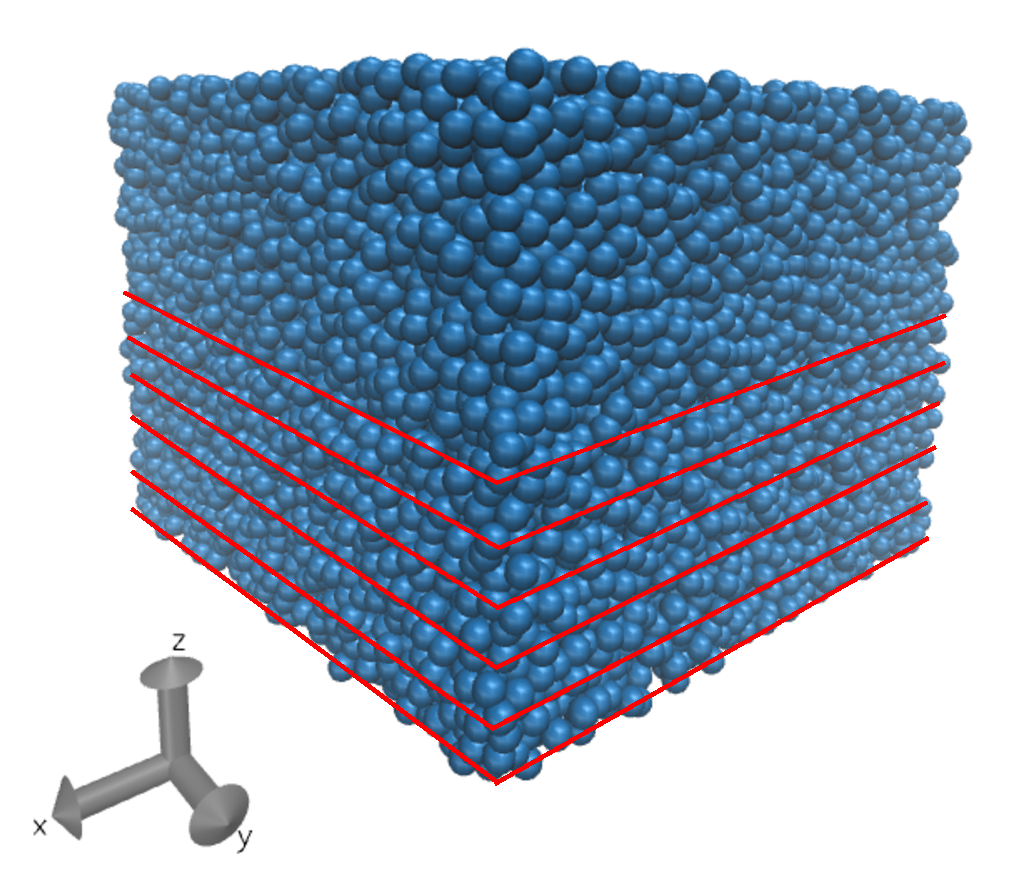
\includegraphics[scale=0.3]{system_nodes_periodic}
    \caption[Periodic box]{A visual representation of the MD simulation with a sketch of the binning used. In red are depicted the nodal planes used.}
    \label{fig:PBCBox}
\end{figure}

As CG variables we choose  the set of discrete hydrodynamic
variables,  which are  the  mass density  $\hat{\rho}_\mu(z)$ and  the
momentum  density $\hat{\bf  g}_\mu(z)$  defined at  the nodal  points
$\mu$
\begin{align}
\hat{\rho}_\mu(z)&= \sum_i^Nm_i\delta_\mu({\bf r}_i)
% \nonumber\\
% \hat{e}_\mu(z)&= \sum_i^Ne_i\delta_\mu({\bf r}_i)
\nonumber\\
\hat{\bf g}_\mu(z)&= \sum_i^N{\bf p}_i\delta_\mu({\bf r}_i)
\label{rhogmumic}
\end{align}
where ${\bf r}_i,{\bf p}_i$ are the position and momentum of particle $i$, 
 the discrete Dirac delta function as 
\begin{align}
\delta_\mu({\bf r})&=  \frac{1}{{\cal V}_\mu}\Phi_\mu({\bf r})
\label{delta}
\end{align}
with the volume defined as
\begin{align}
  {\cal V}_\mu&=\int d{\bf r}\Phi_\mu({\bf r}),
\end{align}
and $\Phi_\mu({\bf r})$  is the finite element basis  function, a tent
function centered  at the nodal plane  $\mu$ and that depends  only on
the $z$ component  of ${\bf r}$.  The mass density  at a node receives
information about the  mass of fluid molecule $i$ that  depends on the
distance of this molecule to the  nodal plane $\mu$, and similarly for
the  momentum.   The  microscopic  variables  (\ref{rhogmumic})  give,
essentially, the number  of particles and momentum per  unit volume of
the particles that happen to be ``around'' the nodal plane $\mu$.  The rationale for using this definition has been discussed in Chapter (\ref{Chap:Planar})


Note that the finite  element basis  functions $\Phi_\mu({\bf  r})$  form a
partition of unity, i.e.
\begin{align}
  \sum_\mu\Phi_\mu({\bf r})=1
\label{PartUnit}
\end{align}
The  partition  of unity  implies  that  if  we compute  the  discrete
integral  (i.e. sum  over bins  times the  volume of  the bin)  of the
discrete hydrodynamic variables we obtain
\begin{align}
  \sum_\mu{\cal V}_\mu\hat{\rho}_\mu(z)&  &&= mN
% \nonumber\\
%   \sum_\mu{\cal V}_\mu\hat{e}_\mu(z)&= \sum_i^N\left(\frac{{\bf p}^2_i}{2m_i}+\phi_i\right)&&=\hat{H}(z)
\nonumber\\
  \sum_\mu{\cal V}_\mu\hat{\bf g}_\mu(z)&=\sum_i^N{\bf p}_i&&= \hat{\bf P}_T(z)
\label{DiscCons}
\end{align}
where we  have introduced the total  mass $mN$ and the  total momentum
$\hat{\bf  P}_T(z)$ of  the  system.  These  are  quantities that  are
conserved under  the Hamiltonian  evolution of the  microscopic state.


In this work we  will only  consider the correlations  of the
component  $\hat{g}^1_\mu$ of  the  momentum density  parallel to  the
bins. These variables are collected into the $N_{\rm bin}$-dimensional
vector           $\hat{g}(z)=\{\hat{g}^1_1(z),\cdots,\hat{g}^1_{N_{\rm
    bin}}(z)\}$ of the $x$ component  of the discrete momentum density
of each of the ${N_{\rm bin}}$ bins in which the periodic box has been
divided.  We  have checked  through MD  simulations that  the coupling
between  this  component  and   the  rest  of  hydrodynamic  variables
(density,  other momentum  components) is  negligible.  Therefore,  we
expect  that a  theory  of  just the  transverse  momentum  is a  good
candidate for  a Markovian theory.  
%Sound perpendicular to  walls that
%requires both the mass density  and the perpendicular component of the
%discrete momentum will be considered elsewhere.

\subsection{The dynamics}
\label{Sec:Trans}
The correlation matrix of the  CG variables $\hat{A}$, assumed to have zero
equilibrium average, is 
\begin{align}
  C(t)&=\llangle \hat{A}(t)\hat{A}^T\rrangle
\end{align}
where the $\llangle\cdots\rrangle$ denotes the equilibrium average and
$T$ is for transpose. 

Mori theory for correlations presented in Section (\ref{Sec:Mori}) allows us to obtain the evolution of the matrix of correlations $C(t)$ as
\begin{align}
    \frac{d}{dt}C(t) = -(L+M^*)\cdot C^{-1}(0)\cdot C(t),
\end{align}
where we have use the equations (\ref{AproxC}), (\ref{Lambda}) and the normalized correlation matrix defined as
\begin{align}
  c(t)=C^{-1}(0)\esc C(t)
\end{align}
\Pendiente{Note that the reversible matrix $L$ vanishes because it involves an equilibrium average of a function that is even in the momentum variables}. Therefore
\begin{align}
    \frac{d}{dt}C(t) = -k_BTM^*\cdot c(t)
    \label{AproxCg}
\end{align}
where, in order to make contact  with known results, we have redefined
the transport  matrix $M^*$  by introducing  a prefactor  $k_BT$ where
$k_B$ is Boltzman's constant and $T$ the equilibrium temperature. 
%As a final
%remark, note that the Markovian equation (\ref{AproxCg}) cannot hold at
%$t=0$, because in that case we get $0=-k_BTM^*$, which is non-sense. Clearly,
%such a Markovian equation can only hold beyond certain time $\tau$, related
%to the neglected memory.

\subsection{The Green-Kubo running integral $M(t)$}
The friction matrix $M^*$ in (\ref{GKCorrected}) is
related to the standard Green-Kubo running integral
\begin{align}
M(t)&=\frac{1}{k_BT}\int_0^{t}dt' \llangle i{\cal L}\hat{g}(t')i{\cal L}\hat{g}^T\rrangle
\label{Mmunu}
\end{align}
that  involves the  time
derivative of the  momentum density which, as shown  in Eq. \Pendiente{(\ref{} Versión disceta)}, is
given by
\begin{align}
  i{\cal L}  \hat{g}_{\mu}(z)&=-\frac{\hat{\sigma}^{13}_{\mu}-\hat{\sigma}^{13}_{\mu-1}}{\Delta z}
\label{iLAcurrentx}
\end{align}
This  is a  discrete expression  of the  momentum balance  equation in
which the time rate of change of the momentum of the node $\mu$ is due
to   the   finite   difference   gradient   of   the   stress   tensor
$\hat{\sigma}^{13}_{\mu}$  of  the  neighbour bins.   The 
microscopic   stress   tensor   of  bin $\mu$ is 

\begin{align}
 \hat{ \boldsymbol{\sigma}}_{\mu}
% &=\hat{\bf K}_\mu+\hat{\boldsymbol{\Pi}}_{\mu}
% \nonumber\\
&=
\frac{1}{{\cal V}_\mu} \left[\sum_i{\bf p}_i{\bf v}_i\chi_\mu({\bf r}_i)
+\frac{1}{2}\sum^{N}_{ij}{\bf r}_{ij}\hat{\bf F}_{ij}z_\mu(i,j)\right]
\label{sbin}
\end{align}
where $\chi_\mu({\bf r})$ is the  characteristic function of bin $\mu$
and $z_{\mu}(i,j)$ is the fraction of the distance between atoms $i,j$
that happens to be within bin $\mu$ (\Pendiente{\ref{} Ref.Versión discreta}).

We may write Eq. (\ref{iLAcurrentx}) in matrix form as
\begin{align}
  i{\cal L}\hat{g}&= -B\esc\hat{\sigma}^{13} =F^T\esc\hat{\sigma}^{13}
\label{iLgMat}
\end{align}
where  $\hat{\sigma}$ is  a  $N_{\rm  bin}$-dimensional column  vector
containing the  discrete stress tensor  of bin  $\mu$ and $B$  is the
backward finite difference matrix.  This matrix is $B=-F^T$, where the
matrix $ F$ is the forward finite difference operator (for PBC)
\begin{align}
 {F}=\frac{1}{\Delta z}\left(
    \begin{array}{rrrrr}
-1&1&0&\cdots&0\\
0&-1&1&\cdots&0\\
\vdots      &&\ddots&&\vdots\\
\\
0&\cdots&0&-1&1 
\\
1&\cdots&0&0&-1 \end{array}
\right)
\label{Dforward}
\end{align}
By using (\ref{iLgMat}) into the Green-Kubo integral matrix $M(t)$ in (\ref{Mmunu})
we have
\begin{align}
  M(t)=F^T\esc\eta(t)\esc F
\label{Mtfef}
\end{align}
where  the  \textit{non-local  viscosity  Green-Kubo  matrix}  is  the
running  time integral  of the  correlation  of the  stress tensor  at
different bins,
\begin{align}
  \eta(t) &=\frac{1}{k_BT}\int_0^{t}dt' 
  \llangle \hat{\sigma}^{13}(t')\hat{\sigma}^{13}\rrangle
\label{non-loc}
\end{align}
Note that  for a homogeneous system  (as one with PBC),  the non-local
viscosity    matrix   is    translationally    invariant,   this    is
$\eta_{\mu\nu}=\eta(|\mu-\nu|)$.  This kind  of matrices  commute with
the forward differencing matrix
\begin{align}
  F\esc\eta(t)=\eta(t)\esc F
\label{commute}
\end{align}
By using this commutation property 
 in the Green-Kubo
integral (\ref{Mtfef}) we obtain
\begin{align}
  M(t)=-\Delta\esc \eta(t)
\label{MmunuMat}
\end{align}
where we have introduced  the discrete Laplacian matrix (for PBC) as
\begin{align}
\Delta&\equiv  B\esc F
=\frac{1}{\Delta z^2}\left(
    \begin{array}{rrrrr}
-2&1&0&\cdots&1\\
1&-2&1&\cdots&0\\
\vdots      &&\ddots&&\vdots\\
\\
1&\cdots&0&1&-2    \end{array}
\right)
\end{align}

Note that the Green-Kubo integral (\ref{Mmunu}) can also be written
in the form
\begin{align}
    M(t)&= \frac{1}{k_BT} \int_0^t dt'\frac{d}{dt'}\llangle \hat{g}(t') i{\cal L}\hat{g}^T\rrangle
\nonumber\\
&= \frac{1}{k_BT} \llangle \hat{g}(t) i{\cal L}\hat{g}^T\rrangle
=  -\frac{1}{k_BT}\frac{d}{dt}\llangle \hat{g}(t) \hat{g}^T\rrangle=-\frac{1}{k_BT}\frac{d}{dt}C(t)
\label{E1}
\end{align}
Therefore,  Eqs  (\ref{MmunuMat}),(\ref{E1})  lead  to  the  following
\textit{rigorous and exact} result
\begin{align}
\frac{d}{dt}C(t)&= k_BT \Delta\esc \eta(t)
\label{etaExact}
\end{align}
that links the momentum correlation matrix with the stress correlation
matrix.  This  equation shows  that  the  Green-Kubo running  integral
(\ref{non-loc})  for  the viscosity  matrix  $\eta(t)$  cannot have  a
plateau, as it should decay according to the time derivative of $C(t)$
and,  hence, from  (\ref{AproxC})  as the  correlation matrix  $C(t)$
itself.

\subsection{The  friction   matrix  $M^*$  and  the   non-local  shear
  viscosity matrix}
By analogy with  (\ref{MmunuMat}), we assume that the  friction matrix $M^*$ in
(\ref{AproxCg}) has the structure
\begin{align}
  M^*=-\Delta\esc \eta^*
\end{align}
for a  certain  matrix  $\eta^*$  referred to  as  the  non-local  shear
viscosity  matrix.  The Markovian  dynamics  (\ref{AproxCg})
becomes
\begin{align}
\frac{d}{dt}C(t)&=  k_BT\Delta\esc \eta^*\esc c(t)
\label{AproxCg1}
\end{align}
We  would like  to  obtain  the matrix  $\eta^*$  from the  Green-Kubo
running  integral   (\ref{non-loc})  for  $\eta(t)$.    Comparison  of
(\ref{AproxCg1}) and (\ref{etaExact}) gives
\begin{align}
 \Delta\esc \eta(t) &=\Delta\esc \eta^*\esc c(t)
\label{etaExact1}
\end{align}
If   the   two   matrices    $\Delta,c(t)$   were   invertible,   then
(\ref{AproxCg1}) would  allow to obtain $\eta^*$  from the correlation
of  the  momentum  density,  while Eq.  (\ref{etaExact1})  would  give
$\eta^*$  from the  correlation of  the  stress. Both  routes are,  of
course, mathematically equivalent.  However, both the Laplacian matrix
$\Delta$  and  the  normalized   correlation  matrix  $c(t)$  are  not
invertible.  The reason is that the normalized ``constant'' vector
\begin{align}
  v&=\frac{1}{\sqrt{M}}(1,1,\cdots,1)
\end{align}
is the unique eigenvector of null eigenvalue of the Laplacian operator
with periodic boundary conditions, $\Delta  \cdot v=0$. This vector is
also  eigenvector  of  null   eigenvalue  of  the  correlation  matrix
$C(t)\esc v=0$  due to total momentum  conservation in PBC. 
%Que no tengan un autovalor nulo es condición necesaria para que una matriz sea invertible.
%These two  matrices are
%not invertible, although they are so in the subspace normal to $v$. It is 
%much easier to deal with this issue in Fourier space.
In the next section we take advantage of the periodicity and the translational invariance of the system in order to deal with that issue in Fourier space. 

\subsection{Fourier space}
Consider the unitary matrix with elements
\begin{align}
E_{\mu\nu}=\frac{1}{\sqrt{N_{\rm bin}}}\exp\left\{i\frac{2\pi}{N_{\rm bin}}\mu\nu\right\}
\end{align} 
This matrix has the following inverse
\begin{align}
E^{-1}_{\mu\nu}=\frac{1}{\sqrt{N_{\rm bin}}}\exp\left\{-i\frac{2\pi}{N_{\rm bin}}\mu\nu\right\}
\end{align} 
The indices  are assumed  to run  in the  range $\mu=0,1,\cdots,N_{\rm
  bin}-1$.  
We define the Fourier transform $\tilde{A}$ of a matrix $A$ as
\begin{align}
    \tilde{A}&=E^{-1}\esc A\esc{E}
 \end{align}
with the inverse relation 
 \begin{align}
     A&=E\esc  \tilde{A}\esc{E}^{-1}
\label{FT}
\end{align}
The discrete Laplace operator diagonalizes in Fourier space, this is
\begin{align}
  E^{-1}  \esc {\Delta} \esc E= \tilde{\Delta}
\label{EDE}
\end{align}
where $\tilde{\Delta}$ is a diagonal matrix whose diagonal  elements are
\begin{align}
\tilde{\Delta}_{\mu\mu}&=-\frac{2}{\Delta z^2}
\left(1-\cos\left( \frac{2\pi \mu}{N_{\rm bin}}\right)\right)\le0  
\label{Dmumu}
\end{align}
This is the  spectrum of the discrete Laplace  operator $\Delta$. 


The matrix $E$ diagonalizes any traslation invariant and periodic
matrix    $A_{\mu\nu}$    satisfying    $A_{\mu\nu}=a(|\mu-\nu|)$    and
$a(\mu)=a(N_{\rm bin}-1-\mu)$ as it is easily seen
\begin{align}
&\left[  E^{-1}\esc A\esc E\right]_{\mu\nu}
\nonumber\\
&=
\frac{1}{N_{\rm bin}}\sum_{\mu'=0}^{N_{\rm bin}-1}\sum_{\nu'=0}^{N_{\rm bin}-1} e^{-i\frac{2\pi}{N_{\rm bin}}\mu\mu'}a(|\mu'-\nu'|)
e^{i\frac{2\pi}{N_{\rm bin}}\nu'\nu}
 \nonumber\\
&=\frac{1}{N_{\rm bin}}\delta_{\mu\nu}\underbrace{\sum_{\sigma=0}^{N_{\rm bin}-1}a(\sigma)e^{i\frac{2\pi}{N_{\rm bin}}\sigma\nu}}_{\tilde{a}(\nu)}
\end{align}

Because  the  matrix  $C(t)$  is periodic  traslation  invariant,  the
Fourier     transform     is     a    diagonal     periodic     matrix
$\tilde{C}_{\mu\nu}(t)=\delta_{\mu\nu}\tilde{C}_{\mu\mu}(t)$.
The two equations (\ref{AproxCg1}),(\ref{etaExact1}) become in Fourier space
\begin{align}
  \frac{d}{dt}\tilde{C}(t)&=  k_BT\tilde{\Delta}\esc \tilde{\eta}^*\esc \tilde{c}(t)
\nonumber\\
 \tilde{\Delta}\esc \tilde{\eta}(t) &=\tilde{\Delta}\esc \tilde{\eta}^*\esc \tilde{c}(t)
\label{Fou1}
\end{align}
All matrices  appearing in  these equations are  diagonal.  Therefore,
except  for $\mu=0$,  where $\tilde{c}_{00}=0$  due to  total momentum
conservation,  we  may  infer  the  diagonal  elements  of  the  shear
viscosity matrix in Fourier space  $\tilde{\eta}^*$ from either any of
these two equations
\begin{align}
  \tilde{\eta}^*_{\mu\mu}&= \frac{1}{ k_BT\tilde{\Delta}_{\mu\mu}  \tilde{c}_{\mu\mu}(t)}\frac{d}{dt}\tilde{C}_{\mu\nu}(t)
\nonumber\\
\tilde{\eta}_{\mu\mu}^*&=\frac{\tilde{\eta}_{\mu\mu}(t) }{\tilde{c}_{\mu\mu}(t)}
\label{FouFin}
\end{align}
These two expressions are mathematically  equivalent but they allow to
obtain   the    non-local   shear    viscosity   in    Fourier   space
$\tilde{\eta}_{\mu\mu}^*$ either  from the correlation of  momemtum or
from the  correlation of stress.   The existence  of a plateau  in the
time-dependent  functions of  the  right hand  side in  (\ref{FouFin})
constitute both, a validation of  the Markovian assumption, as well as
a way to computate the non-local shear viscosity.

If we wish  to recover the non-local shear viscosity  in real space we
need   to  know   all   their  eigenvalues.    However,  the   element
$\tilde{\eta}_{00}$  cannot be  computed  from (\ref{FouFin})  because
$\tilde{c}_{00}=0$.  Note that this value  can be obtained directly by
recognizing that
\begin{align}
    \tilde{\eta}_{00}(t)&=E_{0\mu}^{-1}\cdot\eta_{\mu\nu}(t)\cdot E_{\nu 0}=\frac{1}{N_{\rm bin}}
\sum_{\mu\nu}\eta_{\mu\nu}(t)
\label{eta00}
\end{align}
From
(\ref{sbin}) and the fact that $\chi_\mu({\bf r}),z_{\mu}(i,j)$ form a partition of unity, we have
that the total stress is the arithmetic average of the stress in each bin is given by
\begin{align}
\hat{\sigma}_T^{13}=\frac{1}{N_{\rm bin}}\sum_\mu\hat{\sigma}_\mu^{13}
\label{TotStress2}
\end{align}
where the  total stress $\hat\sigma_T^{13}$ is defined  in the usual way
\begin{align}
\hat{\sigma}_T^{13}&=\frac{1}{V_T}\left[\sum_{i}{\bf p}^1_i{\bf v}^3_i
+\frac{1}{2}\sum_{ij}{\bf r}^1_{ij}\hat{\bf F}^3_{ij}\right]
\label{TotStress}
\end{align}
and $V_T$ is the total volume of the system. 

By using (\ref{non-loc}) in (\ref{eta00}) we obtain
\begin{align}
    \tilde{\eta}_{00}(t)&=\frac{1}{N_{\rm bin}}\frac{1}{k_BT}\int_0^tdt'\llangle \sum_{\mu}\hat{\sigma}^{13}_{\mu}(t')\sum_{\nu}\hat{\sigma}^{13}_{\nu}\rrangle
\end{align}
Using the Eq. (\ref{TotStress2})
\begin{align}
    \tilde{\eta}_{00}(t)&=\frac{N_{\rm bin}}{k_BT}\int_0^tdt'\llangle \hat{\sigma}^{13}_T(t')\hat{\sigma}^{13}_T\rrangle
\end{align}
Introducing the \textit{local}  shear viscosity given by the standard Green-Kubo
integral
\begin{align}
  \eta_0(t) &\equiv \frac{V_T}{k_BT}\int_0^t dt'\llangle \hat{\sigma}_T^{13}(t')\hat{\sigma}_T^{13}
\rrangle
\label{etat}
\end{align}
we finally reach 
\begin{align}
    \tilde{\eta}_{00}(t)=\frac{N_{\rm bin}}{V_T}\eta_0(t)
\end{align}
Therefore, the eigenvalue $\tilde{\eta}_{00}(t)$ can be computed independently from
the local shear viscosity.

\subsection{The non-local kinematic viscosity matrix}
It is convenient to introduce the non-local kinematic viscosity matrix
$\nu^*$ as  the non-local shear  viscosity matrix $\eta^*$  divided by
some ``mass density''. As we will see, the notion of locality in space
is best addressed with the kinematic  viscosity and that is the reason
of introducing it here. In  a discrete setting, the connection between
the  discrete momentum  and  the discrete  velocity  is slightly  more
involved than  in the continuum  for which  one has the  simple result
${\bf g}({\bf  r})=\rho({\bf r}){\bf  v}({\bf r})$.  In  the discrete,
the proportionality  between velocity and  momentum is through  a mass
density \textit{matrix} \cite{3}.  Let us see the details.

\Pendiente{As  shown  in Appendix  \ref{Ap:Cov},  the  covariance $C(0)$  of  the
discrete momentum density in PBC is given by
\begin{align}
C_{\mu\nu}(0)&= \frac{k_BT}{{\cal V}_\mu} \rho_{\mu\nu}
\label{gg}
\end{align}
where we have introduced the mass density matrix $\rho_{\mu\nu}$ as
\begin{align}
  \rho_{\mu\nu}&\equiv  m{\cal V}_\mu n \left[ M^\delta_{\mu\nu}-
\frac{1}{n N}  \llangle \hat{n}_\mu\hat{n}_\nu\rrangle\right]
\label{MassMat}
\end{align}
where  $\hat{n}_\mu=\hat{\rho}_\mu/m$ is  the number  density  of node $\mu$ and $n=N/V$  is the  average
number density.  The
matrix $M^\delta_{\mu\nu}$ is
\begin{align}
  M^\delta_{\mu\nu}&=\int d{\bf r}\delta_\mu({\bf r})\delta_\nu({\bf r}) 
\end{align}
For a system  with regular bins with constant volume  ${\cal V}$ each,
this matrix takes the form
\begin{align}
{M}^\delta&=\frac{1}{6{\cal V}}
\left(\begin{array}{cccccc}
4&1&0&\cdots &0&1\\
1&4&1&\cdots &0&0\\
\vdots&&&\ddots&&\vdots\\
0&0&0&\cdots &4&1\\
1&0&0&\cdots&1&4
\end{array}\right)
\end{align}
The last  term in (\ref{MassMat}) scales  as the inverse of  the total
number  $N$ of  particles and  it is  negligible in  the thermodynamic
limit.  However, we  should keep it as it  has observable consequences
in  our simulations.   In fact,  this  term is  responsible for  total
momentum conservation (\ref{DiscCons}), this is
\begin{align}
  \sum_\mu{\cal V}_\mu\llangle \hat{g}_\mu\hat{g}_\nu\rrangle &=0
\end{align}
as   it   should,   because    the   total   momentum   $\sum_\mu{\cal
  V}_\mu\hat{g}_\mu$ vanishes  in the  center of mass  reference frame
that we take.
} %Fin pendiente


By using the explicit form (\ref{gg}) of the covariance matrix, we may
express Eq. (\ref{AproxCg1}) in the form
\begin{align}
\frac{d}{dt}C(t)= \Delta\esc \nu^*\esc C(t)
\label{SDECpi}
\end{align}
where we  have introduced  the non-local  \textit{kinematic} viscosity
matrix through the matrix
\begin{align}
\nu^*&\equiv  \eta^*\esc{\cal V}\esc \rho^{-1}
\label{nustar}
\end{align}
where ${\cal  V}$ is a diagonal  matrix that contains in  the diagonal
the volume ${\cal  V}_\mu$ of the bins.   In Fourier space Eq. (\ref{nustar})
takes the diagonal form
\begin{align}
  \tilde{\nu}_\mu^*&=  \frac{{\cal V}_\mu \tilde{\eta}_\mu^*}{\tilde{\rho}_\mu}
\end{align}
We now show why we refer to the matrix $\eta^*$ as the non-local shear
viscosity  and  to  the  matrix $\nu^*$  as  the  non-local  kinematic
viscosity.   According   to  Mori  theory,  which   encompass  Onsager
regression  hypothesis, the  evolution  of the  average  value of  the
discrete momentum should evolve according to a vector equation analogous to
(\ref{SDECpi}) for the correlation matrix
\begin{align}
  \frac{d}{dt}g(t)&={\cal V}\esc \Delta\esc\eta^*\esc v(t)
%   \frac{d}{dt}g(t)&=\Delta\esc
% \eta^*\esc k_BTC^{-1}(0)\esc g(t)
\label{dgDnug}
\end{align}
where we have defined the discrete velocity field $v$ according to

\Note{A partir de aquí se añade un superíndice al momento y a la velocidad que lo mismo no es necesario poner }
\begin{align}
  v_\mu&\equiv\sum_\nu \rho_{\mu\nu}^{-1}g^1_\nu
\label{vel}
\end{align}
The matrix  $\rho_{\mu\nu}$ defined in (\ref{MassMat})  has dimensions
of a mass density and it  is fairly diagonal.  Its inverse $\rho^{-1}$
is concentrated on the diagonal (in fact, it decays exponentially fast
as we move out from the diagonal).  Because of this, we may interprete
$v_\mu$ defined in (\ref{vel}) as a velocity that contains information
about   the   discretization   method   used.    The components of
Eq. (\ref{dgDnug}) are
\begin{align}
  \frac{d}{dt}{g}_\mu(t)&=
-\sum_\nu{\cal V}_\nu 
\frac{\left[
\eta^*_{\mu+1\nu}-2\eta^*_{\mu\nu}+\eta^*_{\mu-1\nu}\right]}{\Delta z^2}{v}_\nu^1(t)
\end{align}
where we have used the translation invariance of the viscosity matrix.
By a suitably rellabeling  of indices we have
\begin{align}
  \frac{d}{dt}{g}_\mu(t)&=\sum_\nu{\cal V}_\nu \eta^*_{\mu\nu}
\frac{\left[{v}_{\nu+1}^1-2{v}_{\nu}^1+{v}_{\nu-1}^1\right]}{\Delta z^2}
\label{SDELap0} 
\end{align}

Eq. (\ref{SDELap0}) looks    like    a   discretization    of    the    following
integro-differential  equation
\begin{align}
  \frac{d}{dt} g^1(z)&=\int dz'{\eta}^*(z-z')\partial^2_{z'} v^1(z')
\label{congx}
\end{align}
This is  a non-local generalization  of the diffusion equation  of the
continuum transverse  momentum,
\begin{align}
  \partial_t g^1(z)&=\nu^*_0\partial^2_{z}g^1(z')
\label{congx3}
\end{align}
Eq.   (\ref{congx3})   is  obtained  from  (\ref{congx})   by  setting
$\eta^*(z-z')=\eta^*_0\delta(z-z')$,   where   the   local   kinematic
viscosity is  $\nu^*_0=\eta^*_0/\rho$.  Therefore, it is  justified to
refer to the matrix $\eta^*_{\mu\nu}$ introduced in (\ref{non-loc}) as
the  non-local shear  viscosity matrix  and to  $v_\mu$ introduced  in
(\ref{vel}) as the velocity.


\subsection{The local in time prediction}
By using (\ref{EDE})  and (\ref{Dmumu}), the Fourier  transform of the
equation of motion (\ref{SDECpi}) is then
\begin{align}
  \frac{d\tilde{C}_\mu}{dt}(t)&=-\frac{1}{\tau_\mu}\tilde{C}_\mu(t)  
\label{SDECpiDiag}
\end{align}
where the correlation time is given by 
\begin{align}
 \frac{1}{\tau_\mu}&\equiv \frac{2}{\Delta z^2}
\left(1-\cos\left( \frac{2\pi \mu}{N_{\rm bin}}\right)\right)
\tilde{\nu}_\mu^*
\label{taumu}
\end{align}
The  solution of  Eq.  (\ref{SDECpiDiag})  with ``initial  condition''
$\tilde{C}_\mu(\tau)$ at time $\tau$ is the exponential function
\begin{align}
  \tilde{C}_\mu(t)&=\exp\left\{-\frac{t-\tau}{\tau_\mu}\right\}  \tilde{C}_\mu(\tau)
\label{solexp}
\end{align}
The eigenvalues must be decay in an exponential way if the Markovian aproximation is correct. 
The displacement of the initial condition to the time $\tau$ is due to
the fact that  we know that the exponential behaviour  cannot start at
$t=0$  where   the  Markovian  equation  (\ref{AproxC})   and,  hence
(\ref{SDECpiDiag}), cannot hold strictly.

In real space, the correlation matrix is given by Eq. (\ref{SDECpi})
\begin{align}
  C(t)&=\exp\left\{\Delta\esc \nu^* (t-\tau) \right\}C(\tau)
\label{Cmunut}
\end{align}
where the exponential matrix takes the form
\begin{align}
\left[\exp\left\{\Delta\esc \nu^* t \right\}\right]_{\mu\nu}
&=\frac{1}{N_{\rm bin}}\sum_{\mu'}\exp\left\{i\frac{2\pi}{N_{\rm bin}}(\mu-\nu)\mu'\right\}
\nonumber\\
&\times
\exp\left\{-\frac{t}{\tau_{\mu'}}\right\}
\end{align}
In summary, the prediction of the correlation matrix in Fourier space
is given  by single exponentials, while  in real space is  given by a
linear combination of  single exponentials. As we will  see, the later
will give rise to quasi-algebraic decay of correlations.

\subsection{The local in space prediction}
The   discrete   version   of  the   local   continuum   hydrodynamics
Eq. (\ref{congx3}) is simply
\begin{align}
  \frac{d}{dt}{g}_\mu(t)=&\nu_0\Delta_{\mu\nu}{g}_\nu(t)
\label{gloc}
\end{align}
By comparing  this discrete equation  in the local  approximation with
the non-local  discrete equation  (\ref{dgDnug}) we conclude  that the
local approximation of the non-local viscosity matrix $\nu^*$ becomes a
diagonal matrix of the form
\begin{align}
\nu_{\mu\mu'}^*&\simeq \nu_0 \delta_{\mu\mu'}
\end{align}
where the local kinematic viscosity is given by
\begin{align}
\nu_0&\equiv \sum_{\mu'}\nu_{\mu\mu'}^* \quad \quad \quad\forall \mu
\label{nu0}
\end{align}
In the  local approximation, the differential  equation (\ref{SDECpi})
for the correlation matrix becomes
\begin{align}
  \frac{d}{dt}{C}(t)=&\nu_0{\Delta}\esc { C}(t)
\label{LocalEq}
\end{align}
The Fourier transform of the local Eq. (\ref{LocalEq}) is identical to
(\ref{SDECpiDiag})  but  with  a  constant  value  for  the  kinematic
viscosity in (\ref{taumu})
\begin{align}
\tilde{\nu}^*_\mu&= \nu_0
\label{numunu0}
\end{align}
for all $\mu$. Therefore, the  local hydrodynamic prediction says that
the Fourier kinetic viscosity  coefficients $\tilde{\nu}_\mu$ take the
constant value $\nu_0$ given in (\ref{nu0}).
In the local approximation, the relaxation time (\ref{taumu}) is given by 
\begin{align}
 \frac{1}{\tau^{\rm loc}_\mu}&=\frac{2}{\Delta z^2}
\left(1-\cos\left( \frac{2\pi \mu}{N_{\rm bin}}\right)\right)
\nu_0
\label{taumuloc}
\end{align}

%\subsection{Summary of the theory}
%The  two main  quantities of  concern  are the  correlation matrix  of
%discrete momentum  $C(t)$ and the  correlation matrix of  the discrete
%stress  that appears  in  the Green-Kubo  running integral  $\eta(t)$.
%These two  matrices can be measured  from MD simulations. In  order to
%test the locality in time, we use the simple prediction (\ref{solexp})
%for the  eigenvalues of the correlation  matrix. In order to  test the
%non-locality  in space,  from Eq.   (\ref{FouFin}) we  will infer  the
%nonlocal shear viscosity matrix  $\tilde{\eta}^*$ and from the Fourier
%transform   of  (\ref{nustar})   the  non-local   kinematic  viscosity
%$\tilde{\nu}^*$. The local  approximation in space will be  good if we
%can approximate  $\tilde{\nu}^*$ as in (\ref{numunu0}).   Once we have
%measured  $\Lambda^*$  or  equivalently  $\eta^*$ or  $\nu^*$  we  can
%compare  the  prediction  (\ref{Cmunut})  from Mori  theory  with  the
%correlation matrix measured in the simulation.


\section{Simulations}
\label{Sec:Sim}
In Section (\ref{Sec:MoriShearHydro}) we saw that the  two main  quantities of  concern  are the  correlation matrix  of
discrete momentum  $C(t)$ and the  correlation matrix of  the discrete
stress  that appears  in  the Green-Kubo  running integral  $\eta(t)$.
These two  matrices can be measured  from MD simulations. In  order to
test the locality in time, we use the simple prediction (\ref{solexp})
for the  eigenvalues of the correlation  matrix. In order to  test the
non-locality  in space,  from Eq.   (\ref{FouFin}) we  will infer  the
nonlocal shear viscosity matrix  $\tilde{\eta}^*$ and from the Fourier
transform   of  (\ref{nustar})   the  non-local   kinematic  viscosity
$\tilde{\nu}^*$. The local  approximation in space will be  good if we
can approximate  $\tilde{\nu}^*$ as in (\ref{numunu0}).   Once we have
measured  $\Lambda^*$  or  equivalently  $\eta^*$ or  $\nu^*$  we  can
compare  the  prediction  (\ref{Cmunut})  from Mori  theory  with  the
correlation matrix measured in the simulation.

The objective of this section is to present the simulations we made to measure the
momentum  correlation  matrix  $C(t)$  and  the  Green-Kubo  non-local
viscosity $\eta(t)$.   From these primary quantities,  we obtain their
Fourier transforms  $\tilde{C}(t),\tilde{\eta}(t)$ which  are diagonal
matrices  due to  traslation invariance.  

\subsection{Simulation set up}
A  system  of particles  interacting  with  a Lennard-Jones  potential
truncated at  $\sigma=2.5$ has been  simulated in PBC with  the LAMMPS
code.  The box  size is $40\times40\times30$, the  number of particles with mass $m=1$
is $N=28749$, and the time step is $0.002$ in reduced units.  After an
equilibration  of  $10^5$ timesteps  with  a  Langevin thermostate  to
produce a microstate typical  from a thermodynamic point corresponding
to $T=2,\rho=0.6$ in  reduced units, the system is  evolved under NVE
microcanonical conditions for a  further $10^5$ timesteps.  After this
equilibration  phase,  production  runs   of  $15\cdot 10^5$  time  steps  are
launched.   The $z$  axis is  binned  in $60$  bins on  which the  $x$
component of the momentum density is recorded.  The
width of the  bin is $\Delta z=0.5\sigma$ which is  subatomic.  In the
presence of walls,  such a bin allows to resolve  the density layering.  A total of $60\times  60$ correlations corresponding to the
elements of  the correlation matrix  are computed in  each simulation.
The correlations are computed with the LAMMPS command {\it fix ave/correlate}. During $7.5\cdot 10^5$ time steps the $x$ component of the momentum density is recorded every $2$ time steps. These values are used to obtain the correlations with a support of $15\cdot10^4$ time steps. %LAMMPS 7500 puntos curva de correlación separados por 2*dt-> soporte de 15000 (i.e. t=30)
After $7.5\cdot 10^5$ steps the correlations are averaged with the previous one. 
In  order to  increase  statistics,  we 
exploit   the   traslation   invariance   of   the
system.  Although computing  all the  correlation matrix  elements may
seem  unnecessary,  we will  use  the  same methodology  for  confined
fluids. In  this later  case, traslation invariance  is broken  and we
need to consider the full correlation matrix.

\subsection{The correlation matrix $C(t)$}

In  Fig. \ref{fig:Ct-matrix-PBC} we  plot the  correlation  matrix of  the
transverse     momentum      $C_{\mu\nu}(t)=\llangle     g^1_{\mu}(t)\
g^1_\nu\rrangle$ at  the time  $t=0$ and $t=0.6$.  This  matrix is  periodic and
traslation invariant.  Therefore, statistical errors have been further
reduced by averaging this matrix ``along diagonals''.  In addition, we
have taken advantadge of the  analytical calculation of the covariance
$\llangle g^1_{\mu} g^1_\nu\rrangle$ in the Appendix \ref{Ap:Cov} in a
manner that we describe below.
\begin{figure}
\centering
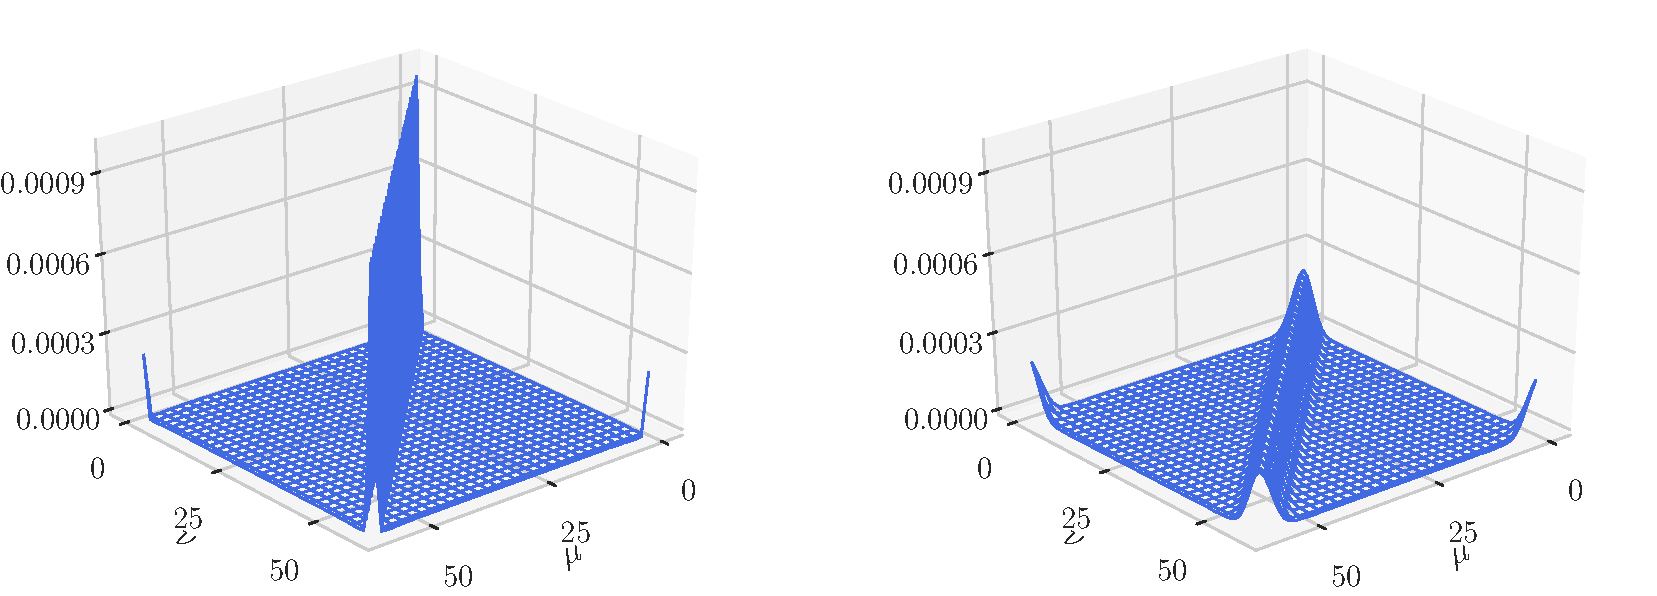
\includegraphics[scale=0.4]{Ct-matrix-PBC}
\caption[Correlation matrix $C(t)$ at $t=0$ and $t=0.6$ for PBC system.]{The   correlation    matrix   $C_{\mu\nu}(t)=\llangle
g_{\mu}(t)  g_\nu\rrangle$ for  $t=0$ (left) and $t=0.6$ (right).}
\label{fig:Ct-matrix-PBC}
\end{figure}

\begin{figure}
\centering
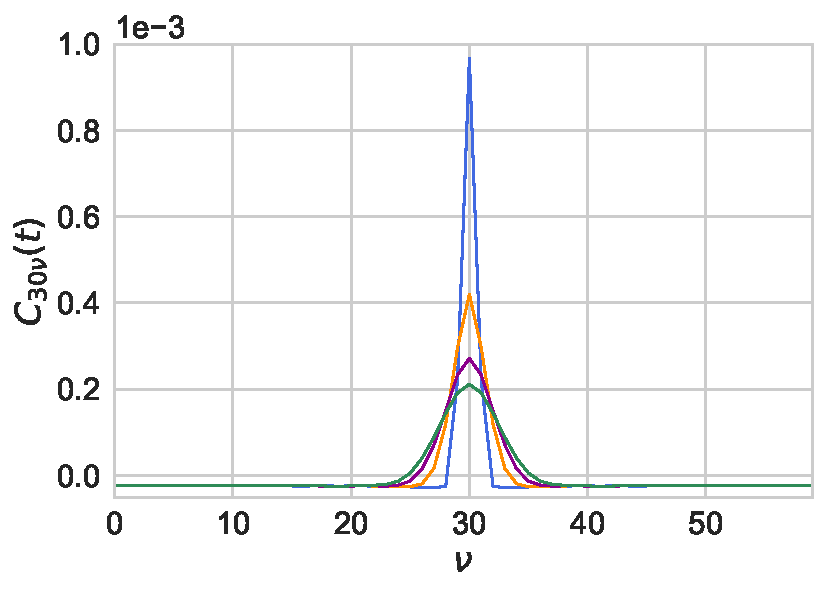
\includegraphics[scale=0.5]{Ct-mu30nu-PBC}
\caption[$C_{30\nu}(t)$ for PBC system.]{$C_{\mu\nu}(t)=\llangle  g^1_{\mu}(t) g^1_\nu\rrangle$  for $\nu=30$
 as a  function of node index  $\nu$ and for times $t=0, 0.2, 0.4, 0.6$ in descending order.  }
 \label{fig:Ct-mu30nu-PBC} 
\end{figure}

\begin{figure}
\centering
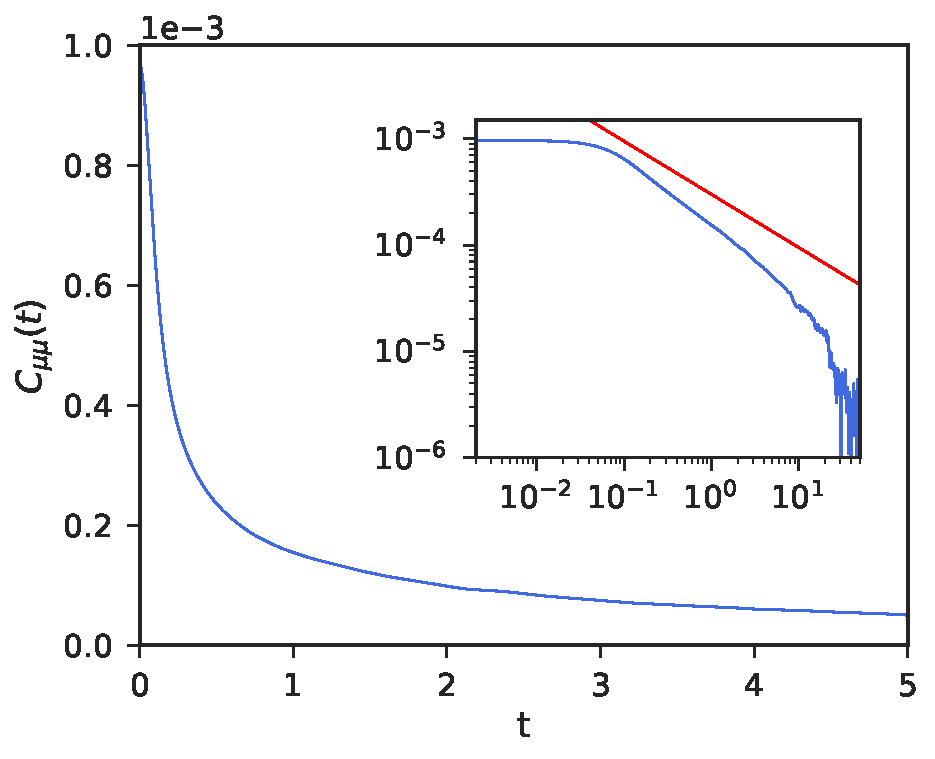
\includegraphics[scale=0.5]{Ct-mu30nu30-PBC}
\caption[Autocorrelation for PBC system.]{The autocorrelation
  $\llangle g_{\mu}(t) g_\mu\rrangle$ (for  any $\mu$)
  . The correlation  decays very
slowly, in an  apparent algebraic way as can be  seen in logscale in the inset.}
  \label{fig:Autocorrelation-PBC}
\end{figure}

In  Fig.    \ref{fig:Ct-mu30nu-PBC}  the   correlations  $\llangle
g^1_{\mu}(t)  g^1_\nu\rrangle$ for  $\mu=30$ and  different values  of
$\nu$ at $t=0, 0.2, 0.4, 0.6, 0.8$ is shown.  This is the row 30 of the matrix plotted
in Fig. \ref{fig:Ct-matrix-PBC}.  We  observe a diffusive
behaviour over  a negative  background.  The  origin of  this negative
global  correlation for  nodes that  are far  appart is  due to  total
momentum conservation in PBC.  If a bin has  a positive momentum, the rest of
bins should  have an  overall negative  value in  order for  the total
momentum to  be zero. In order  to improve the statistical  quality of
the matrix  $C(t)$ we have  used the analytical value  (\ref{Cneg}) of
the  background,  as  provided  by the  analytic  calculation  of  the
covariance in the Appendix \ref{Ap:Cov}.

The autocorrelation $\llangle  g^1_{\mu}(t) g^1_\mu\rrangle$ (which is
the same for  all $\mu$) is shown in  Fig.  \ref{Fig-Autocorrelation-PBC}
as a function of time in both  linear and log scales.  Also shown is a
function $\propto  t^{-1/2}$.  The observed decay  does not correspond
to this algebraic decay.  As discussed in Appendix \ref{Ap:Cont}, only
in both,  the continuum and  thermodynamic limits, we expect  the long
time  tail   $\propto  t^{-1/2}$  behaviour  predicted   by  continuum
hydrodynamics.
\begin{figure}
  \centering
  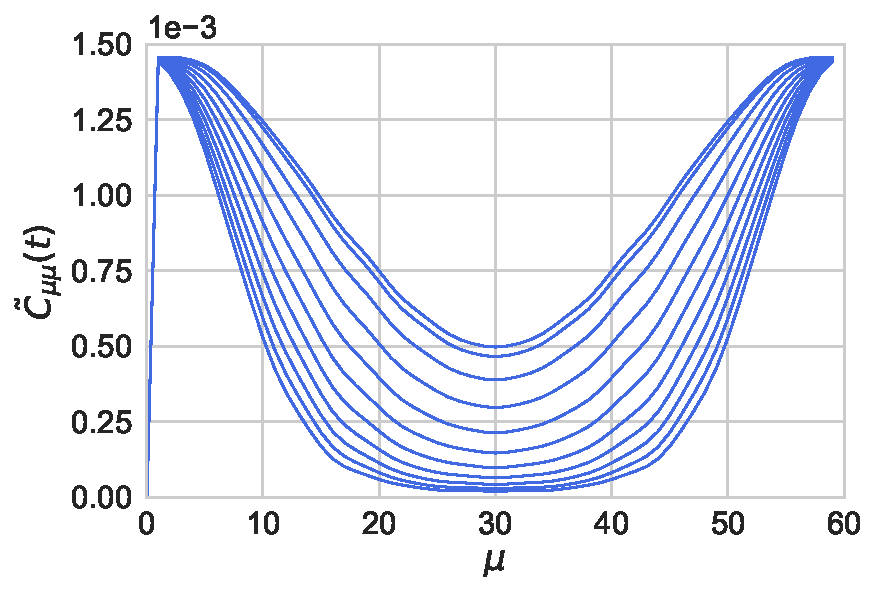
\includegraphics[scale=0.5]{CtFourier-PBC}
  \caption[Diagonal $\tilde{C}_{\mu\nu}(t)$]{The diagonal $\tilde{C}_{\mu\mu}(t)$ of the Fourier transform
  of the correlation  matrix $C(t)$ for different values  of the time.
  In      descending     order      the     plotted      times     are
$t=0.10,0.12,0.14,0.16,0.18,0.20$.}
\label{CtFourier-PBC}
\end{figure}

\begin{figure}
  \centering
  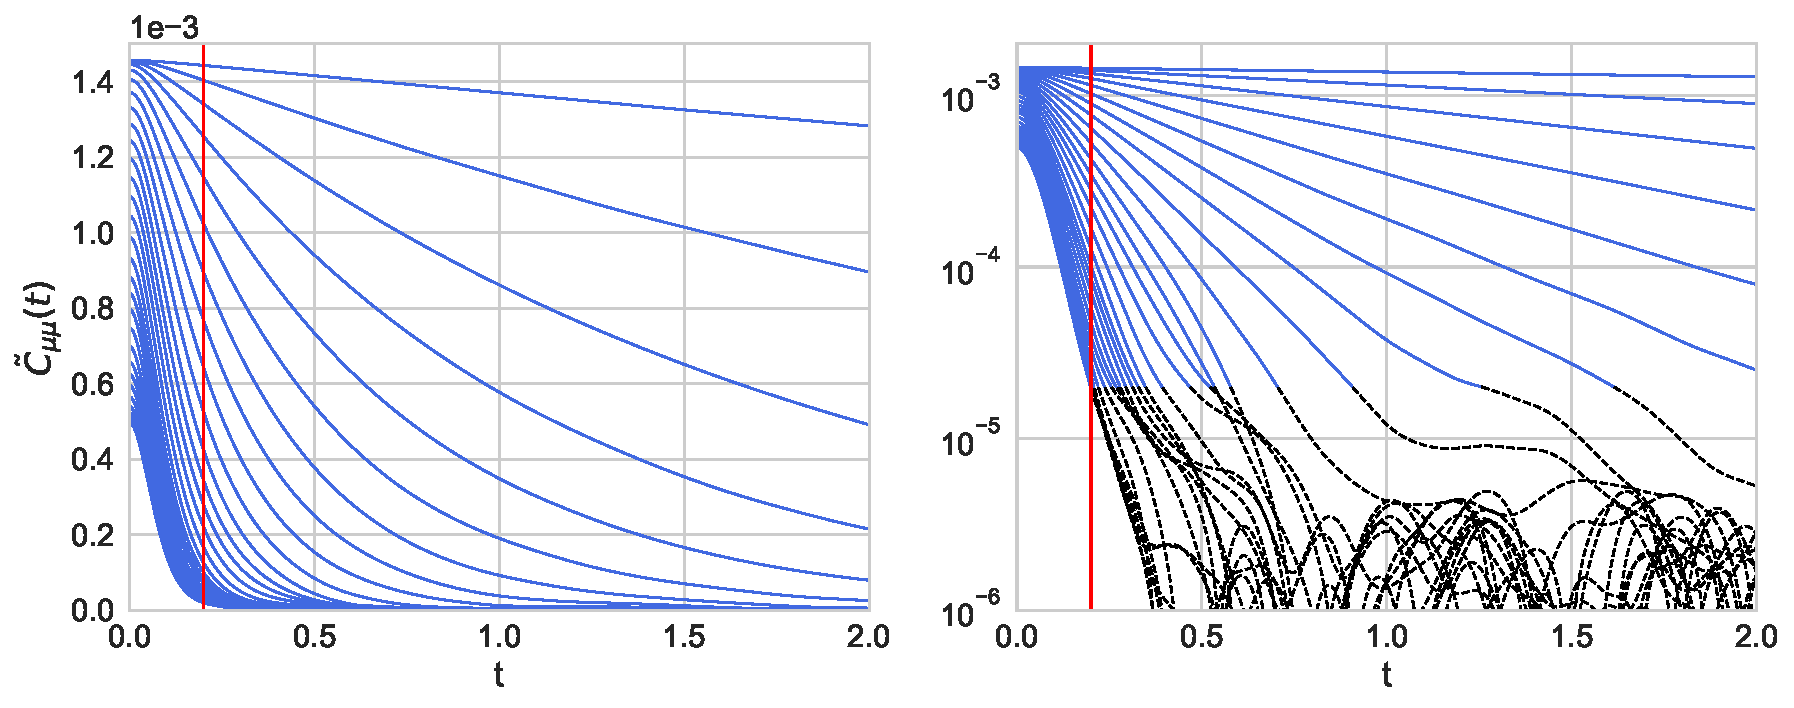
\includegraphics[scale=0.45]{CtFourier-PBC-exp}
  \caption[Evolution of different eigenvalues $\tilde{C}_{\mu\nu}(t)$]{
  In      descending     order      the     plotted      times     go from
  $t=0$ to $t=0.20$ in intervals of $0.02$.  The  evolution of  the different
  eigenvalues  $\tilde{C}_{\mu\mu}(t)$ of  the  correlation matrix  of
  momentum  as  a  function  of   time  in  a  lin-lin  plot  (middle)
  and   log-lin   plot
  (bottom). Also  plotted are  a vertical line  at $t=\tau=0.2$  and a
  horizontal  line  at  the   value  $2\times10^{-5}$,  signaling  the
  threshold below which statistical errors give spurious results. }
\label{CtFourier-PBC-exp}
\end{figure}

The Fourier transform $\tilde{C}(t)$  of the correlation matrix $C(t)$
is a diagonal matrix.  The diagonal $\tilde{C}_{\mu\mu}(t)$ is plotted
in the top panel in Fig.   \ref{Fig-Ct4.eps} as a function of the mode
$\mu$      for      different       values      of      the      time,
$t=0.10,0.12,0.14,0.16,0.18,0.20$  in  descending   order.   The  mode
$\mu=0$ gives a vanishing value  because of momentum conservation.  As
can be seen in Fig.   \ref{Fig-Ct4.eps}, at the largest times plotted,
the  value  of  the  diagonal  correlation  matrix  in  Fourier  space
$\tilde{C}_\mu(t)$ goes to  zero for modes with  values near $\mu=30$,
implying the  amplification of the  statistical errors in  the inverse
matrix in that  region.  In Fig.  \ref{fig:CtFourier-PBC-exp}  middle panel we
plot the  eigenvalues $\tilde{C}_{\mu\mu}(t)$  as a function  of time.
Observe  that after  a time  around  $\tau=0.2$ the  decay in  log-lin
(bottom  panel) is  approximately  linear,  suggesting an  exponential
decay.


\subsection{Validation of the Markov property}
\begin{figure}[h]
  \centering
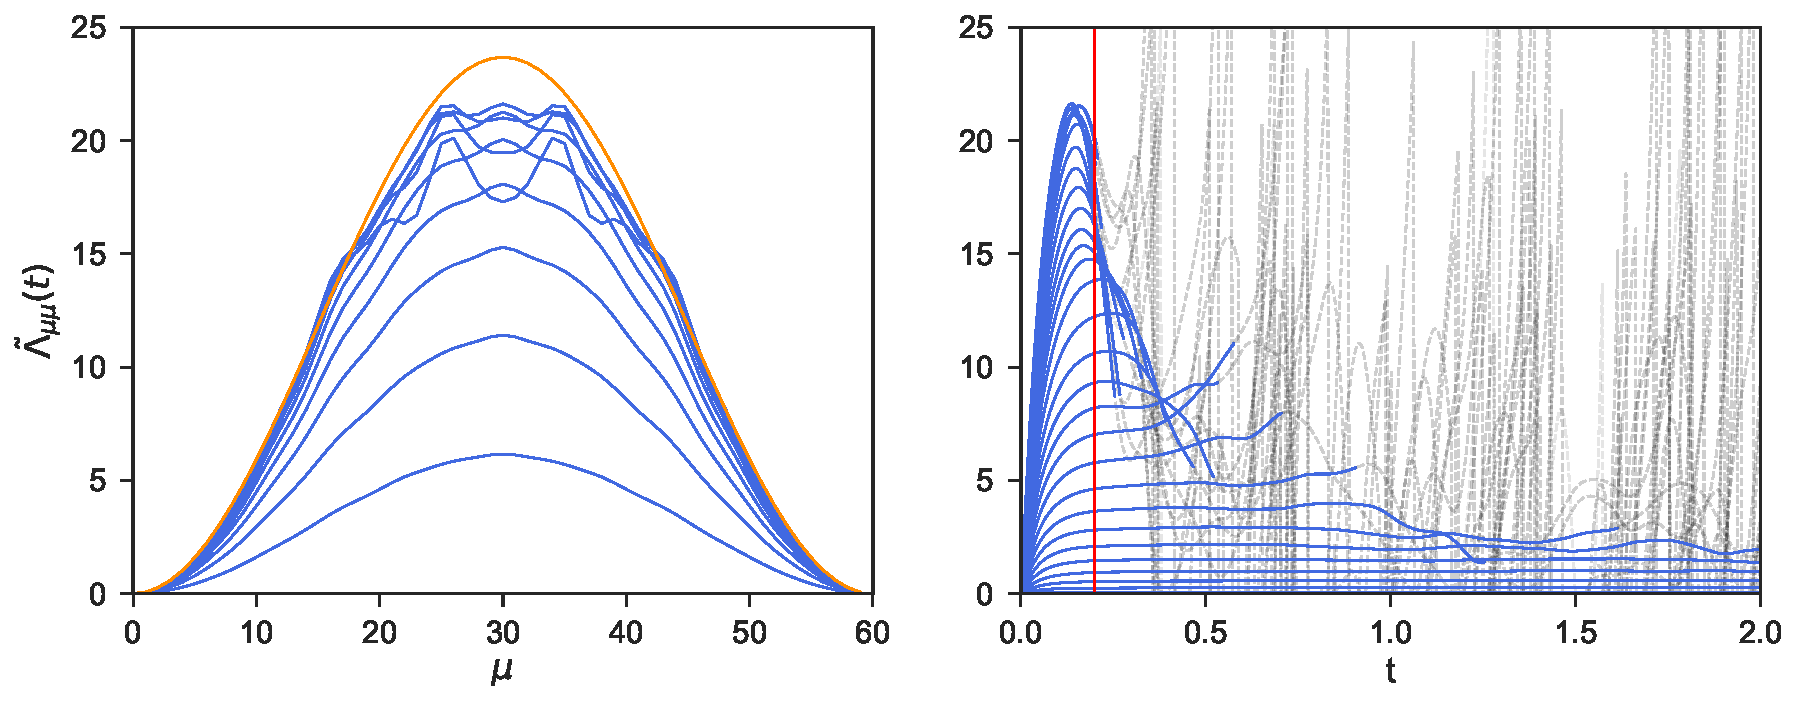
\includegraphics[scale=0.45]{LambdatFourier-PBC}
\caption{The  diagonal elements  $\tilde{\Lambda}_{\mu\mu}(t)$ of  the
  Fourier transform of $\Lambda(t)$ defined in (\ref{AproxCtau}), as a
  function of  $\mu$ (top)  and $t$  (bottom).  In  the top  panel, in
  ascending  order the  plotted times  go  from $t=0$  to $t=0.20$  in
  intervals of $0.02$.  The dotted line is the local approximation Eq.
  (\ref{Lambdaloc}) with a  value of the local  kinematic viscosity of
  $\nu_0=1.48$.   In the  bottom panel,  we observe  a clear  plateau,
  beyond  $\tau=0.2$  indicating  the  exponential  behaviour  of  the
  correlations in Fig. \ref{fig:CtFourier-PBC-exp}.}
\label{fig:LambdatFourier-PBC}
\end{figure}









\begin{figure}
    \centering
    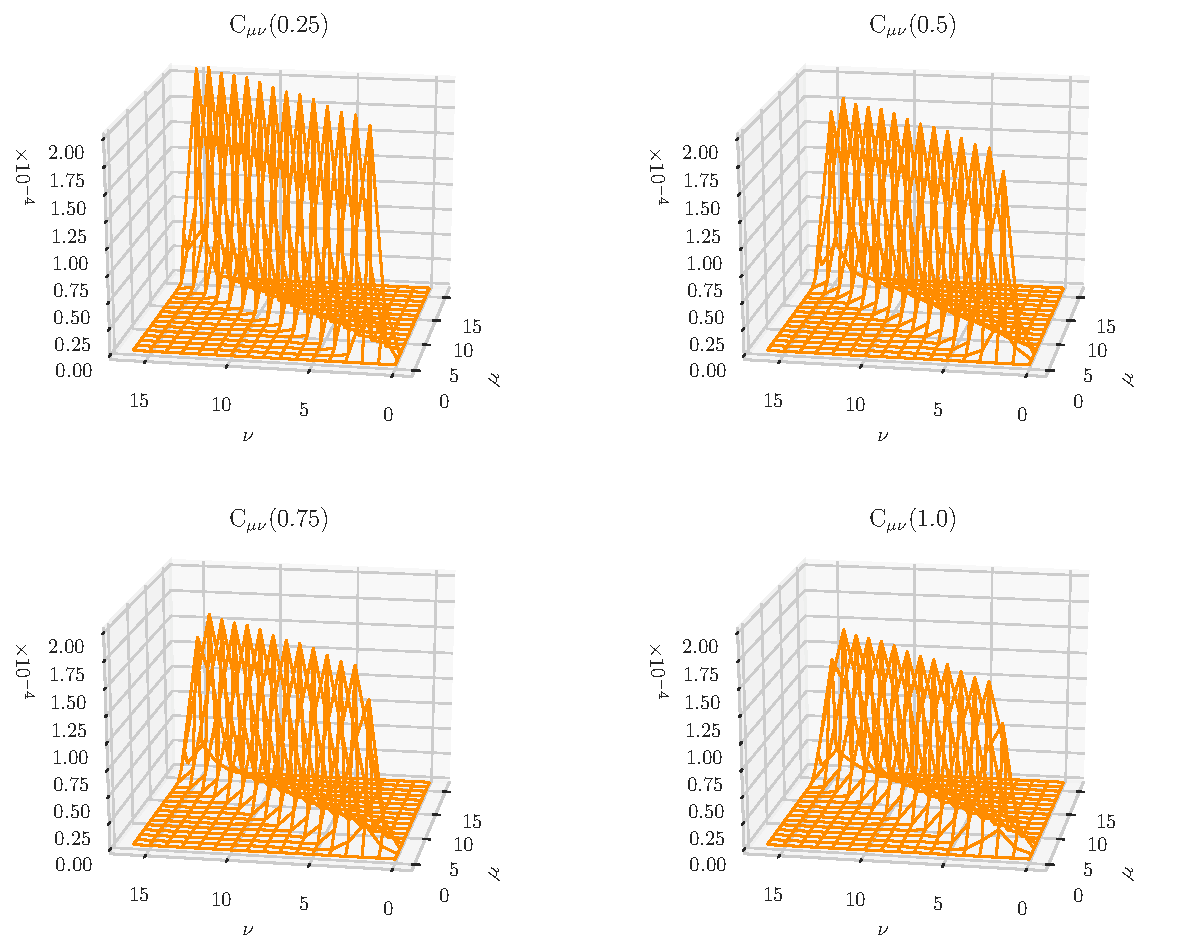
\includegraphics[scale=0.8]{Ct-matrix-17nodes}
    \caption[Snapshots of C(t)]{Matrix $C(t)$ for different times.}
    \label{fig:CtMatrix17Nodes}
\end{figure}

\begin{figure}
    \centering
    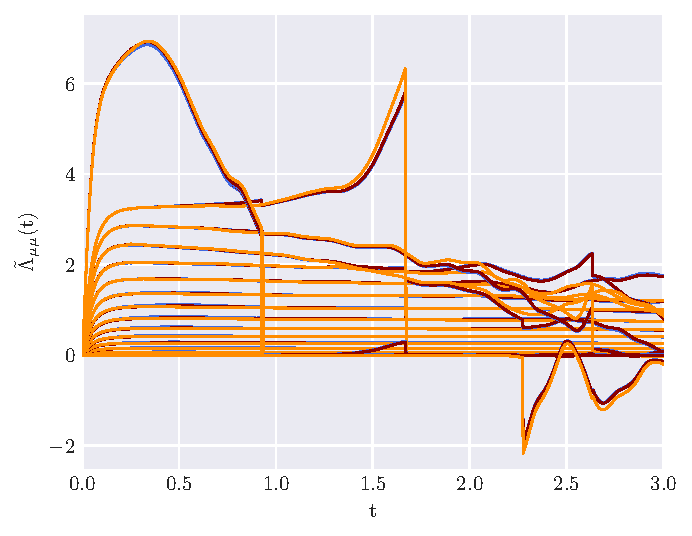
\includegraphics[scale=0.8]{Lambda-17nodes}
    \caption[$\Lambda(t)$ for a system of 17 nodes]{$\Lambda(t)$ for three basis: blue $E(0.15)$, red $E(0.30)$ and orange $E(t)$}
    \label{fig:Lambda17Nodes}
\end{figure}

\begin{figure}
    \centering
    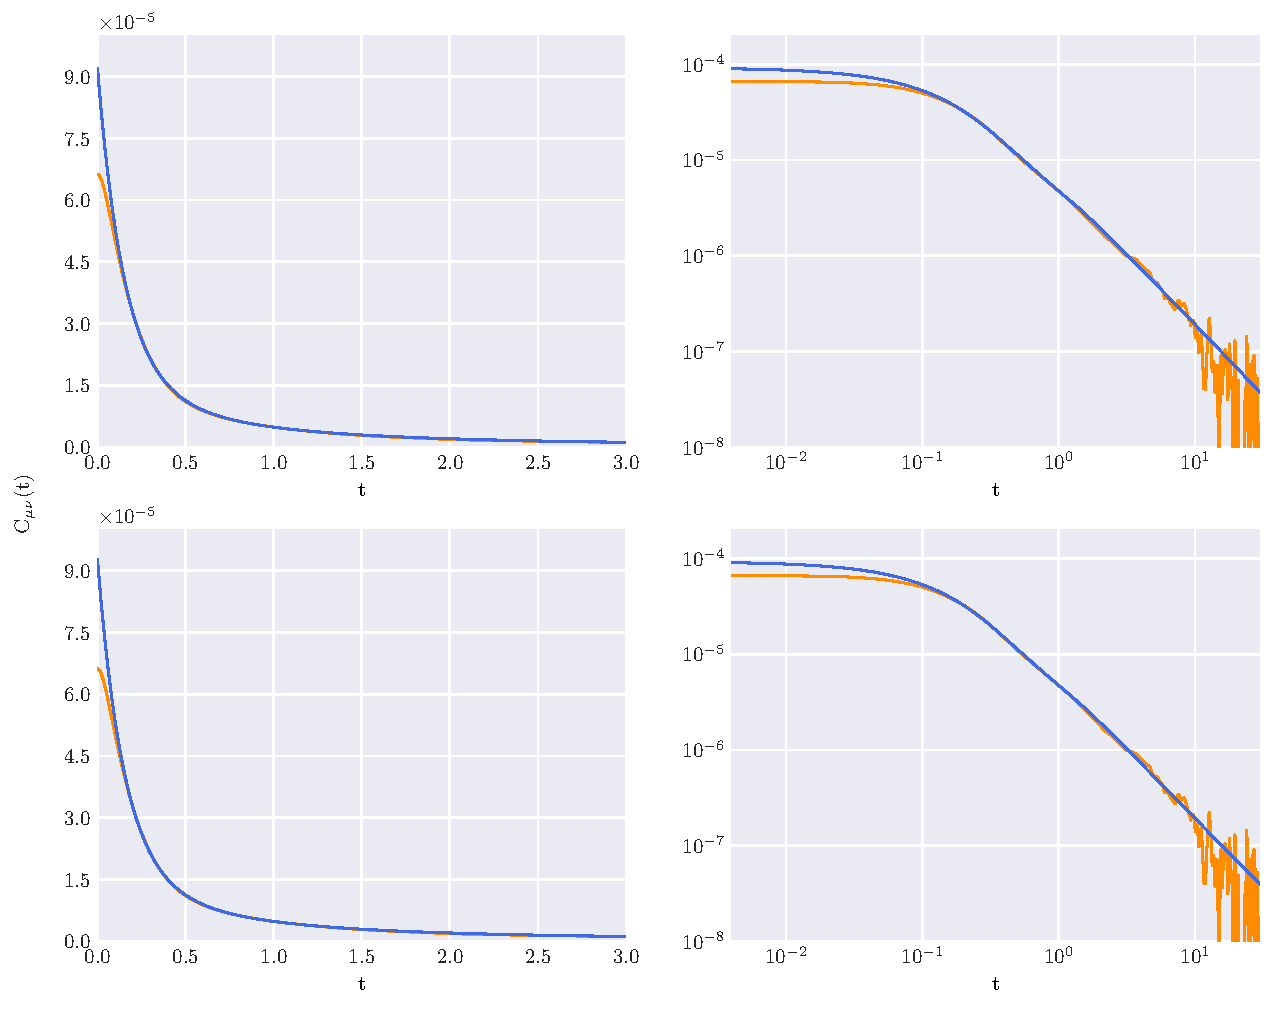
\includegraphics[scale=0.7]{Predictions-17nodes}
    \caption[$C(t)$ predictions for a system of 17 nodes]{In the top panel, in the middle and in the bottom.}
    \label{fig:CtPredictions17Nodes}
\end{figure}


\Note{Cuando tenga que poner las gráficas de las correlaciones y predicciones coger el centro del canal y mu=30, nu=31 con el soporte hasta 10. Están en el directorio ~/Escritorio/lambda/66nodes/PBC con nombre Ct-gxTh-mu30nu31 y Ct-gxTh-mu30nu30. Los he copiado a este directorio por si pierdo esos ficheros.}





\chapter{Correlations of transverse momentum}\label{cap.TransMomentum}
\markboth{Correlation of transverse momentum}{}
\epigraph{\textit{Descubrir es ver de otro modo lo que nadie ha percibido.}}{Blanco Nocturno \\ RICARDO PLIGIA}
\section{Introduction}



\begin{figure}
    \centering
    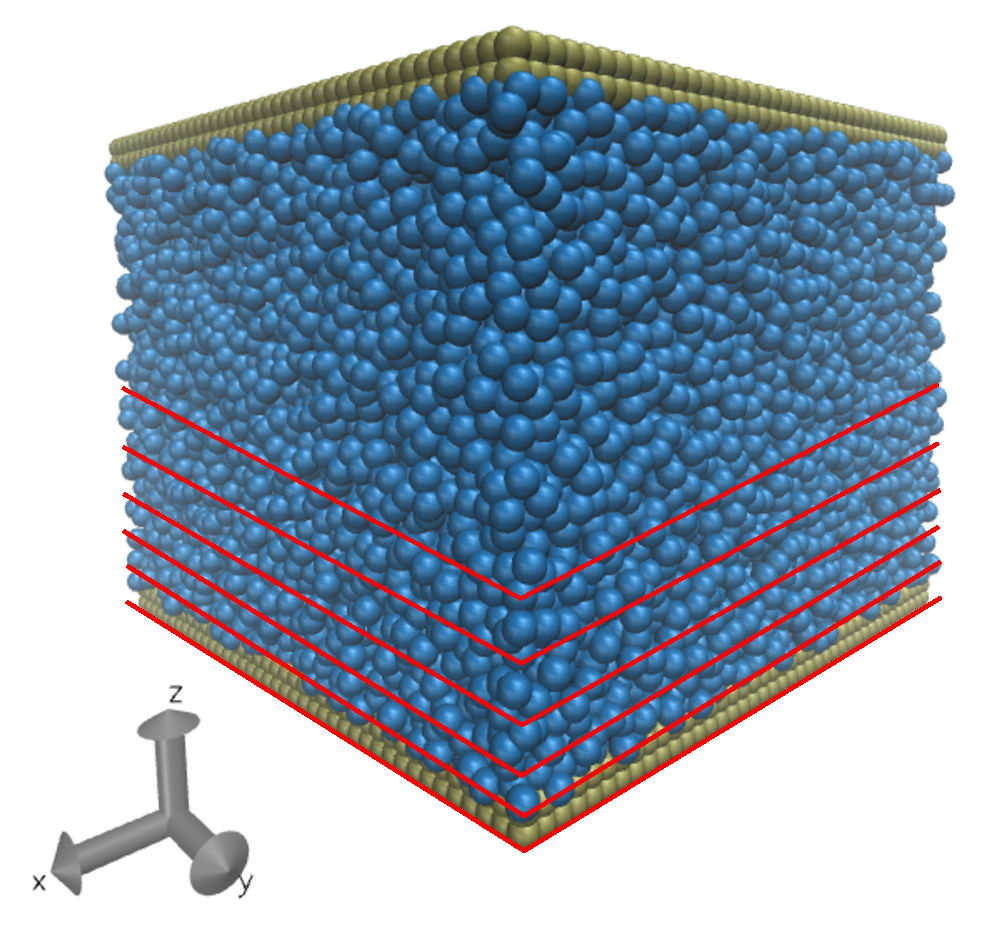
\includegraphics[scale=0.3]{system_nodes_walls}
    \caption[Walls box]{A visual representation of the MD simulation with a sketch of the binning used. In red are depicted the nodal planes used.}
    \label{fig:WallsBox}
\end{figure}
\section{Summary}

\chapter{MD, BC eta estrella y gamma estrella}\label{cap.}
\epigraph{\textit{It is remarkable how long men will believe in the bottomlessness of a pond without taking the trouble to sound it}}{Walden \\ HENRY DAVID THOREAU}
\markboth{Co}{}
\section{Introduction}
\section{Summary}


\chapter{Conclusions}\label{cap.Conclusions}
%\epigraph{\it{El auténtico corredor corre hasta el final.}}{El corredor \\ JOHN L. PARKER}
\section{Summary}

\appendix
\chapter{List of Acronyms}\label{aped.A}
\begin{tabular}{l l}
    CM & Classical Mechanics \\
    FFT & Fast Fourier Transform \\
    GLE & Generalized Langevin Equation \\
    MD & Molecular Dynamics \\
    SM & Statistical Mechanics \\
    ToCG & Theory of Coarse-Graining \\
\end{tabular}

\chapter{Notation, conventions and quotes}\label{aped.B}

Functions of microstates z in phase space are denoted with a hat as in $\hat{A}(z)$. We follow this convention except for probability densities, as in $\rho_t(z)$. Operators are denoted with ${\cal CALIGRAPHIC}$ symbols. Vectors and matrices are denoted with {\bf boldfaces}.
%We use a number of superscripts for matrices. $M^T$ is the transpose of $M$ , $M^S = (M+M^T )/2$ is the symmetric part of the matrix M while $M^A = (M-M^T )/2$ is the antisymmetric part. 


We follow Einstein summation convention in which, for example the product of two matrices in components is written as
\begin{align}
    (AB)_{\mu\nu} = A_{\mu\nu}B_{\nu\sigma}=\sum_{\nu}A_{\mu\nu}B_{\nu\sigma}
\end{align}
The derivative of a composite function is expressed as
\begin{align}
    \frac{\partial}{\partial x}F(g(x))=\frac{\partial F}{\partial g}(g(x))\frac{\partial g}{\partial x}(x)
\end{align}


The quotes in the beginning of each chapter are taken from books I read over the time a spend working in this dissertation, the last four years. I have respected the language in which the writter wrote the novel. 


\section*{Physical parameters and variables}
\begin{tabular}{l l}
    N & Number of particles \\
    M & Number of nodes \\
    $k_B$ & Boltzmann's constant \\
    T & Temperature \\
    $\beta$ & $(k_BT)^{-1}$ \\
\end{tabular}

\chapter{The covariance}
\label{Ap:Cov}
In  this  appendix,  we  compute   explicitly  the  covariance  of  the
transverse momentum density  which is given by  the molecular ensemble
average
\begin{align}
  C_{\mu\nu}^E&=\llangle \hat{g}_\mu^1\hat{g}_\nu^1\rrangle
=\frac{1}{\Omega\left(E\right)}
\int dr dp \delta\left(\hat{H}(z)-E\right)
\delta\left(\sum_i^N{\bf p}_i\right) 
\sum_{ij}^N{\bf p}_i^1{\bf p}_j^1\delta_{\mu}({\bf r}_i) 
\delta_{\nu}({\bf r}_j) 
\end{align}
The molecular ensemble is microcanonical in the total energy and total
momentum, where  we have chosen the  reference frame of the  center of
mass  of the  system, where  total momentum  vanishes.  Although  this
microcanonical average can be computed  explicitly, it is much simpler
to compute the following canonical average
\begin{align}
  C_{\mu\nu}^\beta =\llangle \hat{g}_\mu^1\hat{g}_\nu^1\rrangle
=\frac{1}{Z(\beta)}
\int dr dp \exp\{-\beta\hat{H}(z)\}
\delta\left(\sum_i^N{\bf p}_i\right) 
\sum_{ij}^N{\bf p}_i^1{\bf p}_j^1\delta_{\mu}({\bf r}_i) 
\delta_{\nu}({\bf r}_j) 
\end{align}
where the Dirac delta function on  the Hamiltonian is substituted by a
Gibbs factor. We  keep, however the momentum  conservation Dirac delta
function as this has observable consequences.  The two covariances are
related by
\begin{align}
  C^{\beta}_{\mu\nu}&=\int dE P_\beta(E)
  C^{E}_{\mu\nu}
\end{align}
where the probability distribution of the energy in the canonical ensemble is
\begin{align}
P_\beta(E)&=  \frac{1}{Z(\beta)}e^{-\beta E}\Omega(E)
\end{align}
In the thermodynamic limit, the probability distribution is highly peaked
at the average energy $E^*$ corresponding to the particular value $\beta$. In this case, we may approximate the molecular
ensemble average with the canonical average
\begin{align}
  C^{\beta}_{\mu\nu}&=  C^{E^*}_{\mu\nu}
\end{align}
The momentum integral of the canonical average involves a Gaussian and the
Dirac delta function on total momentum. This integral may be computed by
using the Fourier representation of the Dirac delta function. The result
is
\begin{align}
  \frac{\int dp {\bf p}_i{\bf p}_je^{-\beta\sum_ip_i^2/2m_i}
\delta\left(\sum_k{\bf p}_k\right)}{\int dp e^{-\beta\sum_ip_i^2/2m_i}
\delta\left(\sum_k{\bf p}_k\right)}&=k_BT m_i\left(\delta_{ij}-\frac{1}{N}\right){\bf 1}
\label{momint}\end{align}
This expression satisfies  that if we sum both sides  of this equation
over the  total number of particles  we obtain $0=0$ as  it should, on
momentum conservation considerations.

After performing the momentum integrations with the result (\ref{momint})
we obtain
\begin{align}
  C_{\mu\nu}^\beta&=k_BTm n\int d{\bf r}\delta_\mu({\bf r})\delta_\nu({\bf r})
-\frac{k_BTm}{N}\llangle \hat{n}_\mu\hat{n}_\nu\rrangle^{\beta}
\label{Covmunu}
\end{align}
 In this expression $\hat{n}_\mu=\sum_i\delta_\mu({\bf r}_i)$ is the discrete
number density of node $\mu$ and $n=\llangle \hat{n}_\mu\rrangle$ is the average
number density, which for an homogeneous system is independent on the bin, and
given by $n=N/V$.

Note that the covariance satisfies
\begin{align}
  \sum_\mu {\cal V}_\mu C_{\mu\nu}^\beta=0
\end{align}
which is  a reflection of  momentum conservation.  For nodes  that are
more  than, roughly,  a  couple  of bins  appart,  the  first term  in
(\ref{Covmunu}) is very small, and the covariance takes the value
\begin{align}
  C_{\mu\nu}^\beta\simeq -\frac{k_BTm n^2}{N}
\label{Cneg}
\end{align}
This  value, although  vanishingly  small in  the thermodynamic  limit
$N\to\infty$, is  consistently detectable  in our simulations.  From a
physical point of view it means that if a bin has a positive momentum,
the  rest of  the bins  should have  a negative  momentum in  order to
comply  with  a  zero  total momentum,  resulting  into  the  negative
covariance (\ref{Cneg}).

\cleardoublepage
\addcontentsline{toc}{chapter}{List of figures} % para que aparezca en el indice de contenidos
\listoffigures % indice de figuras

\cleardoublepage
\addcontentsline{toc}{chapter}{List of tables} % para que aparezca en el indice de contenidos
\listoftables % indice de tablas

\bibliographystyle{unsrt}
\bibliography{bibTex/thesis-library}
\end{document}
